\documentclass{book}
\usepackage[a4paper,top=2.5cm,bottom=2.5cm,left=2.5cm,right=2.5cm]{geometry}
\usepackage{makeidx}
\usepackage{natbib}
\usepackage{graphicx}
\usepackage{multicol}
\usepackage{float}
\usepackage{listings}
\usepackage{color}
\usepackage{ifthen}
\usepackage[table]{xcolor}
\usepackage{textcomp}
\usepackage{alltt}
\usepackage{ifpdf}
\ifpdf
\usepackage[pdftex,
            pagebackref=true,
            colorlinks=true,
            linkcolor=blue,
            unicode
           ]{hyperref}
\else
\usepackage[ps2pdf,
            pagebackref=true,
            colorlinks=true,
            linkcolor=blue,
            unicode
           ]{hyperref}
\usepackage{pspicture}
\fi
\usepackage[utf8]{inputenc}
\usepackage{mathptmx}
\usepackage[scaled=.90]{helvet}
\usepackage{courier}
\usepackage{sectsty}
\usepackage{amssymb}
\usepackage[titles]{tocloft}
\usepackage{doxygen}
\lstset{language=C++,inputencoding=utf8,basicstyle=\footnotesize,breaklines=true,breakatwhitespace=true,tabsize=4,numbers=left }
\makeindex
\setcounter{tocdepth}{3}
\renewcommand{\footrulewidth}{0.4pt}
\renewcommand{\familydefault}{\sfdefault}
\hfuzz=15pt
\setlength{\emergencystretch}{15pt}
\hbadness=750
\tolerance=750
\begin{document}
\hypersetup{pageanchor=false,citecolor=blue}
\begin{titlepage}
\vspace*{7cm}
\begin{center}
{\Large Baka\-Plan \\[1ex]\large 0.\-6 }\\
\vspace*{1cm}
{\large Generated by Doxygen 1.8.1.2}\\
\vspace*{0.5cm}
{\small Fri Feb 22 2013 23:07:20}\\
\end{center}
\end{titlepage}
\clearemptydoublepage
\pagenumbering{roman}
\tableofcontents
\clearemptydoublepage
\pagenumbering{arabic}
\hypersetup{pageanchor=true,citecolor=blue}
\chapter{Ba\-Ka\-Plan}
\label{md_README}
\hypertarget{md_README}{}
Seating Plan is a project for alotting seat for examination.

This folder consists of all backend proccessing.

\#\-Requirements\-: 1) G\-C\-C Compiler for C++  2) Configure C\-G\-I for executing html pages on browser. 

Language\-: C++ and C\-G\-I for Front End. 

\#\-How to run Download code and then run make command in terminal. 
\chapter{Class Index}
\section{\-Class \-Hierarchy}
\-This inheritance list is sorted roughly, but not completely, alphabetically\-:\begin{DoxyCompactList}
\item \contentsline{section}{\-Database}{\pageref{de/d03/classDatabase}}{}
\item \contentsline{section}{\-Data\-Sheet}{\pageref{dd/dcc/classDataSheet}}{}
\item \contentsline{section}{\-Exapand\-Roll\-No}{\pageref{d2/d9b/classExapandRollNo}}{}
\item \contentsline{section}{\-Input\-Detail}{\pageref{db/d6e/classInputDetail}}{}
\begin{DoxyCompactList}
\item \contentsline{section}{\-Class\-Detail}{\pageref{d9/ddf/classClassDetail}}{}
\item \contentsline{section}{\-Date\-Sheet}{\pageref{de/d0e/classDateSheet}}{}
\item \contentsline{section}{\-Exam\-Detail}{\pageref{df/d4d/classExamDetail}}{}
\begin{DoxyCompactList}
\item \contentsline{section}{\-Valid\-Strategy}{\pageref{d9/d15/classValidStrategy}}{}
\end{DoxyCompactList}
\item \contentsline{section}{\-Login}{\pageref{dd/dfd/classLogin}}{}
\begin{DoxyCompactList}
\item \contentsline{section}{\-Project\-Detail}{\pageref{d3/dd8/classProjectDetail}}{}
\end{DoxyCompactList}
\item \contentsline{section}{\-Report}{\pageref{da/da8/classReport}}{}
\item \contentsline{section}{\-Roll\-No\-Detail}{\pageref{d6/db0/classRollNoDetail}}{}
\item \contentsline{section}{\-Room\-Detail}{\pageref{d4/de5/classRoomDetail}}{}
\item \contentsline{section}{\-Strategy}{\pageref{d2/df2/classStrategy}}{}
\end{DoxyCompactList}
\item \contentsline{section}{\-Input\-Field\-Name}{\pageref{dd/db2/classInputFieldName}}{}
\item \contentsline{section}{\-Java\-Script}{\pageref{da/dac/classJavaScript}}{}
\item \contentsline{section}{\-Page\-Structure\-Maker}{\pageref{de/d88/classPageStructureMaker}}{}
\begin{DoxyCompactList}
\item \contentsline{section}{\-Page\-Layout}{\pageref{d7/d9e/classPageLayout}}{}
\end{DoxyCompactList}
\item \contentsline{section}{\-Read\-Input}{\pageref{de/d50/classReadInput}}{}
\begin{DoxyCompactList}
\item \contentsline{section}{\-Arrange\-Roll\-No}{\pageref{da/de9/classArrangeRollNo}}{}
\begin{DoxyCompactList}
\item \contentsline{section}{\-Date\-Sheet}{\pageref{de/d0e/classDateSheet}}{}
\end{DoxyCompactList}
\item \contentsline{section}{\-Expand\-Roll\-No}{\pageref{d0/d6e/classExpandRollNo}}{}
\item \contentsline{section}{\-Seat\-Plan}{\pageref{d2/d41/classSeatPlan}}{}
\begin{DoxyCompactList}
\item \contentsline{section}{\-Strategy}{\pageref{d2/df2/classStrategy}}{}
\end{DoxyCompactList}
\end{DoxyCompactList}
\item \contentsline{section}{\-Read\-Input\-Field}{\pageref{d8/d37/classReadInputField}}{}
\item \contentsline{section}{\-Send\-Mail}{\pageref{d6/d66/classSendMail}}{}
\end{DoxyCompactList}

\chapter{Class Index}
\section{Class List}
Here are the classes, structs, unions and interfaces with brief descriptions\-:\begin{DoxyCompactList}
\item\contentsline{section}{\hyperlink{classArrangeRollNo}{Arrange\-Roll\-No} }{\pageref{classArrangeRollNo}}{}
\item\contentsline{section}{\hyperlink{classBranchDetails}{Branch\-Details} }{\pageref{classBranchDetails}}{}
\item\contentsline{section}{\hyperlink{classBranchReport}{Branch\-Report} }{\pageref{classBranchReport}}{}
\item\contentsline{section}{\hyperlink{classExamDetails}{Exam\-Details} }{\pageref{classExamDetails}}{}
\item\contentsline{section}{\hyperlink{classExapandRollNo}{Exapand\-Roll\-No} }{\pageref{classExapandRollNo}}{}
\item\contentsline{section}{\hyperlink{classHome}{Home} }{\pageref{classHome}}{}
\item\contentsline{section}{\hyperlink{classHomeCSS}{Home\-C\-S\-S} }{\pageref{classHomeCSS}}{}
\item\contentsline{section}{\hyperlink{classHTMLTags}{H\-T\-M\-L\-Tags} \\*Base class containong Basic Html Tags and methods }{\pageref{classHTMLTags}}{}
\item\contentsline{section}{\hyperlink{classReadBranchDetails}{Read\-Branch\-Details} }{\pageref{classReadBranchDetails}}{}
\item\contentsline{section}{\hyperlink{classReadExamDetails}{Read\-Exam\-Details} }{\pageref{classReadExamDetails}}{}
\item\contentsline{section}{\hyperlink{classReadInput}{Read\-Input} }{\pageref{classReadInput}}{}
\item\contentsline{section}{\hyperlink{classReadRollNoDetails}{Read\-Roll\-No\-Details} }{\pageref{classReadRollNoDetails}}{}
\item\contentsline{section}{\hyperlink{classReadRoomDetails}{Read\-Room\-Details} }{\pageref{classReadRoomDetails}}{}
\item\contentsline{section}{\hyperlink{classReport}{Report} }{\pageref{classReport}}{}
\item\contentsline{section}{\hyperlink{classRollNoDetails}{Roll\-No\-Details} }{\pageref{classRollNoDetails}}{}
\item\contentsline{section}{\hyperlink{classRoomDetails}{Room\-Details} }{\pageref{classRoomDetails}}{}
\item\contentsline{section}{\hyperlink{classRoomReport}{Room\-Report} }{\pageref{classRoomReport}}{}
\item\contentsline{section}{\hyperlink{classSeatPlan}{Seat\-Plan} }{\pageref{classSeatPlan}}{}
\item\contentsline{section}{\hyperlink{classStrategy}{Strategy} }{\pageref{classStrategy}}{}
\item\contentsline{section}{\hyperlink{classSubjectWiseRollNo}{Subject\-Wise\-Roll\-No} }{\pageref{classSubjectWiseRollNo}}{}
\item\contentsline{section}{\hyperlink{classValidation}{Validation} }{\pageref{classValidation}}{}
\end{DoxyCompactList}

\chapter{Class Documentation}
\hypertarget{classArrangeRollNo}{\section{\-Arrange\-Roll\-No \-Class \-Reference}
\label{classArrangeRollNo}\index{\-Arrange\-Roll\-No@{\-Arrange\-Roll\-No}}
}


\-Arrange roll no class for sorting, removing redundant roll nos and also excludeing roll nos that are not for seating plan.  




{\ttfamily \#include $<$arrangerollno.\-h$>$}

\-Inheritance diagram for \-Arrange\-Roll\-No\-:\begin{figure}[H]
\begin{center}
\leavevmode
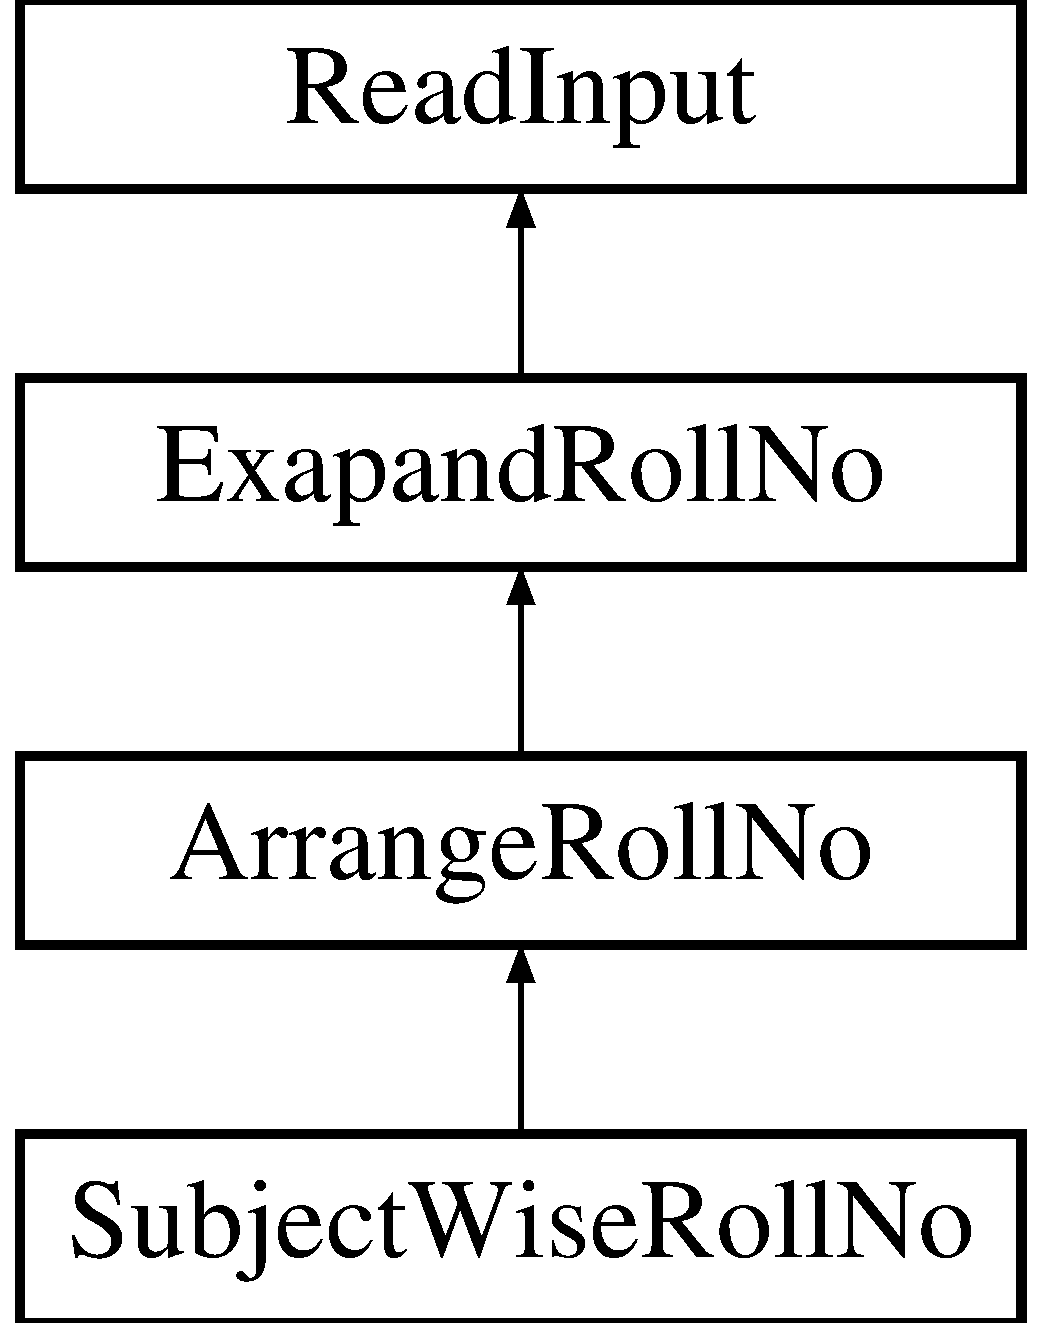
\includegraphics[height=3.000000cm]{classArrangeRollNo}
\end{center}
\end{figure}
\subsection*{\-Public \-Member \-Functions}
\begin{DoxyCompactItemize}
\item 
\hyperlink{classArrangeRollNo_a430515990d97ffa02b65ed5d15d79c9f}{\-Arrange\-Roll\-No} ()
\begin{DoxyCompactList}\small\item\em \-Constructor. \end{DoxyCompactList}\item 
void \hyperlink{classArrangeRollNo_aae9734fb7b98d980d3f1feb1b52a6195}{\-Sort\-Roll\-No} (\-I\-N\-T\-\_\-\-V\-E\-C \&rollno)
\begin{DoxyCompactList}\small\item\em \-Function for sorting roll no vector array. \end{DoxyCompactList}\item 
void \hyperlink{classArrangeRollNo_ab0b6350a9113b86925133d7199929020}{\-Remove\-Redundancy} (\-I\-N\-T\-\_\-\-V\-E\-C \&rollno)
\item 
void \hyperlink{classArrangeRollNo_adeb652c1977c668d2cd519c1a4f317bd}{\-Remove\-Non\-Eligible\-Roll\-No} (\-I\-N\-T\-\_\-\-V\-E\-C \&rollno, \-I\-N\-T\-\_\-\-V\-E\-C \&\hyperlink{classArrangeRollNo_a1f6740950e3180731b74c3ecdc19b98c}{not\-Included\-R\-No})
\begin{DoxyCompactList}\small\item\em \-Removing roll no that are not eligible. \end{DoxyCompactList}\item 
void \hyperlink{classArrangeRollNo_a69151212acbfeb90780b066ade988418}{\-Add\-Prefix\-With\-Roll\-No} (\-I\-N\-T\-\_\-\-V\-E\-C \&rollno, \-S\-T\-R\-I\-N\-G\-\_\-\-V\-E\-C \&\hyperlink{classArrangeRollNo_ac70b1f6e601cc5786ef339a38ae18c6f}{prefix})
\begin{DoxyCompactList}\small\item\em \-Adding prefix with roll nos. \end{DoxyCompactList}\item 
void \hyperlink{classArrangeRollNo_a12e17989e12519e37083b7f5649ebbec}{\-Write\-Arranged\-Roll\-No} ()
\begin{DoxyCompactList}\small\item\em \-Writing arranged roll nos to file as \-O/p file. \end{DoxyCompactList}\item 
void \hyperlink{classArrangeRollNo_a795fde3b512631e07d7189138b39b775}{\-Main} (string p\-I\-D)
\begin{DoxyCompactList}\small\item\em \-Main function to call all functions. \end{DoxyCompactList}\item 
\hyperlink{classArrangeRollNo_acbdaa06590d381ec19a7a07c718b9282}{$\sim$\-Arrange\-Roll\-No} ()
\begin{DoxyCompactList}\small\item\em \-Destructor. \end{DoxyCompactList}\end{DoxyCompactItemize}
\subsection*{\-Protected \-Attributes}
\begin{DoxyCompactItemize}
\item 
\-I\-N\-T\-\_\-\-V\-E\-C \hyperlink{classArrangeRollNo_ad75d3ee3f709606da5b4871098c3e978}{roll\-No}
\item 
\-I\-N\-T\-\_\-\-V\-E\-C \hyperlink{classArrangeRollNo_a1f6740950e3180731b74c3ecdc19b98c}{not\-Included\-R\-No}
\item 
\hypertarget{classArrangeRollNo_ab39f82c658365388d106b3dcc18e69fb}{\-I\-N\-T\-\_\-\-V\-E\-C {\bfseries roll\-No\-Size}}\label{classArrangeRollNo_ab39f82c658365388d106b3dcc18e69fb}

\item 
\hypertarget{classArrangeRollNo_a728b87c54815f5393e93da5909ed90b2}{\-I\-N\-T\-\_\-\-V\-E\-C {\bfseries not\-Included\-R\-No\-Size}}\label{classArrangeRollNo_a728b87c54815f5393e93da5909ed90b2}

\item 
\-S\-T\-R\-I\-N\-G\-\_\-\-V\-E\-C \hyperlink{classArrangeRollNo_ac70b1f6e601cc5786ef339a38ae18c6f}{prefix}
\item 
\-S\-T\-R\-I\-N\-G\-\_\-2\-D\-V\-E\-C \hyperlink{classArrangeRollNo_aa0401159b5d59c7afe77980a391a9a0a}{prefix\-Roll\-No}
\item 
\hyperlink{classExpandRollNo}{\-Expand\-Roll\-No} \hyperlink{classArrangeRollNo_a7ddd59b57f85cf6fea265d38c284df92}{expand\-R\-No}
\end{DoxyCompactItemize}


\subsection{\-Detailed \-Description}
\-Arrange roll no class for sorting, removing redundant roll nos and also excludeing roll nos that are not for seating plan. 

\-Include \hyperlink{arrangerollno_8h}{arrangerollno.\-h} file

\-Include \hyperlink{expandrollno_8h}{expandrollno.\-h} file 

\-Definition at line 30 of file arrangerollno.\-h.



\subsection{\-Constructor \& \-Destructor \-Documentation}
\hypertarget{classArrangeRollNo_a430515990d97ffa02b65ed5d15d79c9f}{\index{\-Arrange\-Roll\-No@{\-Arrange\-Roll\-No}!\-Arrange\-Roll\-No@{\-Arrange\-Roll\-No}}
\index{\-Arrange\-Roll\-No@{\-Arrange\-Roll\-No}!ArrangeRollNo@{\-Arrange\-Roll\-No}}
\subsubsection[{\-Arrange\-Roll\-No}]{\setlength{\rightskip}{0pt plus 5cm}{\bf \-Arrange\-Roll\-No\-::\-Arrange\-Roll\-No} (
\begin{DoxyParamCaption}
{}
\end{DoxyParamCaption}
)}}\label{classArrangeRollNo_a430515990d97ffa02b65ed5d15d79c9f}


\-Constructor. 

\-Constructor 

\-Definition at line 27 of file arrangerollno.\-cc.

\hypertarget{classArrangeRollNo_acbdaa06590d381ec19a7a07c718b9282}{\index{\-Arrange\-Roll\-No@{\-Arrange\-Roll\-No}!$\sim$\-Arrange\-Roll\-No@{$\sim$\-Arrange\-Roll\-No}}
\index{$\sim$\-Arrange\-Roll\-No@{$\sim$\-Arrange\-Roll\-No}!ArrangeRollNo@{\-Arrange\-Roll\-No}}
\subsubsection[{$\sim$\-Arrange\-Roll\-No}]{\setlength{\rightskip}{0pt plus 5cm}{\bf \-Arrange\-Roll\-No\-::$\sim$\-Arrange\-Roll\-No} (
\begin{DoxyParamCaption}
{}
\end{DoxyParamCaption}
)}}\label{classArrangeRollNo_acbdaa06590d381ec19a7a07c718b9282}


\-Destructor. 

\-Desrtuctor 

\-Definition at line 212 of file arrangerollno.\-cc.



\subsection{\-Member \-Function \-Documentation}
\hypertarget{classArrangeRollNo_a69151212acbfeb90780b066ade988418}{\index{\-Arrange\-Roll\-No@{\-Arrange\-Roll\-No}!\-Add\-Prefix\-With\-Roll\-No@{\-Add\-Prefix\-With\-Roll\-No}}
\index{\-Add\-Prefix\-With\-Roll\-No@{\-Add\-Prefix\-With\-Roll\-No}!ArrangeRollNo@{\-Arrange\-Roll\-No}}
\subsubsection[{\-Add\-Prefix\-With\-Roll\-No}]{\setlength{\rightskip}{0pt plus 5cm}void {\bf \-Arrange\-Roll\-No\-::\-Add\-Prefix\-With\-Roll\-No} (
\begin{DoxyParamCaption}
\item[{\-I\-N\-T\-\_\-\-V\-E\-C \&}]{roll\-No, }
\item[{\-S\-T\-R\-I\-N\-G\-\_\-\-V\-E\-C \&}]{prefix}
\end{DoxyParamCaption}
)}}\label{classArrangeRollNo_a69151212acbfeb90780b066ade988418}


\-Adding prefix with roll nos. 

\-Adding prefix with roll nos


\begin{DoxyParams}{\-Parameters}
{\em roll\-No} & \-List of eligible roll nos \\
\hline
{\em prefix} & \-Prefix ie added with roll nos \\
\hline
\end{DoxyParams}


\-Definition at line 107 of file arrangerollno.\-cc.

\hypertarget{classArrangeRollNo_a795fde3b512631e07d7189138b39b775}{\index{\-Arrange\-Roll\-No@{\-Arrange\-Roll\-No}!\-Main@{\-Main}}
\index{\-Main@{\-Main}!ArrangeRollNo@{\-Arrange\-Roll\-No}}
\subsubsection[{\-Main}]{\setlength{\rightskip}{0pt plus 5cm}void {\bf \-Arrange\-Roll\-No\-::\-Main} (
\begin{DoxyParamCaption}
\item[{string}]{p\-I\-D}
\end{DoxyParamCaption}
)}}\label{classArrangeRollNo_a795fde3b512631e07d7189138b39b775}


\-Main function to call all functions. 

\-Main method to call all function in order/sequence


\begin{DoxyParams}{\-Parameters}
{\em p\-I\-D} & \-Project \-I\-D \\
\hline
\end{DoxyParams}


\-Reimplemented in \hyperlink{classDateSheet_af749306c14297b5c93c16f48f551d5bb}{\-Date\-Sheet}.



\-Definition at line 151 of file arrangerollno.\-cc.

\hypertarget{classArrangeRollNo_adeb652c1977c668d2cd519c1a4f317bd}{\index{\-Arrange\-Roll\-No@{\-Arrange\-Roll\-No}!\-Remove\-Non\-Eligible\-Roll\-No@{\-Remove\-Non\-Eligible\-Roll\-No}}
\index{\-Remove\-Non\-Eligible\-Roll\-No@{\-Remove\-Non\-Eligible\-Roll\-No}!ArrangeRollNo@{\-Arrange\-Roll\-No}}
\subsubsection[{\-Remove\-Non\-Eligible\-Roll\-No}]{\setlength{\rightskip}{0pt plus 5cm}void {\bf \-Arrange\-Roll\-No\-::\-Remove\-Non\-Eligible\-Roll\-No} (
\begin{DoxyParamCaption}
\item[{\-I\-N\-T\-\_\-\-V\-E\-C \&}]{roll\-No, }
\item[{\-I\-N\-T\-\_\-\-V\-E\-C \&}]{not\-Included\-R\-No}
\end{DoxyParamCaption}
)}}\label{classArrangeRollNo_adeb652c1977c668d2cd519c1a4f317bd}


\-Removing roll no that are not eligible. 

\-Removing non eligible roll nos


\begin{DoxyParams}{\-Parameters}
{\em roll\-No} & roll nos for seating plan \\
\hline
{\em not\-Included\-R\-No} & \-Roll no list that is not eligible for seating plan \\
\hline
\end{DoxyParams}


\-Definition at line 79 of file arrangerollno.\-cc.

\hypertarget{classArrangeRollNo_ab0b6350a9113b86925133d7199929020}{\index{\-Arrange\-Roll\-No@{\-Arrange\-Roll\-No}!\-Remove\-Redundancy@{\-Remove\-Redundancy}}
\index{\-Remove\-Redundancy@{\-Remove\-Redundancy}!ArrangeRollNo@{\-Arrange\-Roll\-No}}
\subsubsection[{\-Remove\-Redundancy}]{\setlength{\rightskip}{0pt plus 5cm}void {\bf \-Arrange\-Roll\-No\-::\-Remove\-Redundancy} (
\begin{DoxyParamCaption}
\item[{\-I\-N\-T\-\_\-\-V\-E\-C \&}]{rollno}
\end{DoxyParamCaption}
)}}\label{classArrangeRollNo_ab0b6350a9113b86925133d7199929020}
\-Removing redundancy from roll nos 

\-Definition at line 51 of file arrangerollno.\-cc.

\hypertarget{classArrangeRollNo_aae9734fb7b98d980d3f1feb1b52a6195}{\index{\-Arrange\-Roll\-No@{\-Arrange\-Roll\-No}!\-Sort\-Roll\-No@{\-Sort\-Roll\-No}}
\index{\-Sort\-Roll\-No@{\-Sort\-Roll\-No}!ArrangeRollNo@{\-Arrange\-Roll\-No}}
\subsubsection[{\-Sort\-Roll\-No}]{\setlength{\rightskip}{0pt plus 5cm}void {\bf \-Arrange\-Roll\-No\-::\-Sort\-Roll\-No} (
\begin{DoxyParamCaption}
\item[{\-I\-N\-T\-\_\-\-V\-E\-C \&}]{roll\-No}
\end{DoxyParamCaption}
)}}\label{classArrangeRollNo_aae9734fb7b98d980d3f1feb1b52a6195}


\-Function for sorting roll no vector array. 

\-Sorting \-Roll nos


\begin{DoxyParams}{\-Parameters}
{\em roll\-No} & \-For sorting array \\
\hline
\end{DoxyParams}


\-Definition at line 39 of file arrangerollno.\-cc.

\hypertarget{classArrangeRollNo_a12e17989e12519e37083b7f5649ebbec}{\index{\-Arrange\-Roll\-No@{\-Arrange\-Roll\-No}!\-Write\-Arranged\-Roll\-No@{\-Write\-Arranged\-Roll\-No}}
\index{\-Write\-Arranged\-Roll\-No@{\-Write\-Arranged\-Roll\-No}!ArrangeRollNo@{\-Arrange\-Roll\-No}}
\subsubsection[{\-Write\-Arranged\-Roll\-No}]{\setlength{\rightskip}{0pt plus 5cm}void {\bf \-Arrange\-Roll\-No\-::\-Write\-Arranged\-Roll\-No} (
\begin{DoxyParamCaption}
{}
\end{DoxyParamCaption}
)}}\label{classArrangeRollNo_a12e17989e12519e37083b7f5649ebbec}


\-Writing arranged roll nos to file as \-O/p file. 

\-Writing arranged roll no's into file 

\-Definition at line 124 of file arrangerollno.\-cc.



\subsection{\-Member \-Data \-Documentation}
\hypertarget{classArrangeRollNo_a7ddd59b57f85cf6fea265d38c284df92}{\index{\-Arrange\-Roll\-No@{\-Arrange\-Roll\-No}!expand\-R\-No@{expand\-R\-No}}
\index{expand\-R\-No@{expand\-R\-No}!ArrangeRollNo@{\-Arrange\-Roll\-No}}
\subsubsection[{expand\-R\-No}]{\setlength{\rightskip}{0pt plus 5cm}{\bf \-Expand\-Roll\-No} {\bf \-Arrange\-Roll\-No\-::expand\-R\-No}\hspace{0.3cm}{\ttfamily  \mbox{[}protected\mbox{]}}}}\label{classArrangeRollNo_a7ddd59b57f85cf6fea265d38c284df92}
\-Object of \hyperlink{classExpandRollNo}{\-Expand\-Roll\-No} class 

\-Definition at line 45 of file arrangerollno.\-h.

\hypertarget{classArrangeRollNo_a1f6740950e3180731b74c3ecdc19b98c}{\index{\-Arrange\-Roll\-No@{\-Arrange\-Roll\-No}!not\-Included\-R\-No@{not\-Included\-R\-No}}
\index{not\-Included\-R\-No@{not\-Included\-R\-No}!ArrangeRollNo@{\-Arrange\-Roll\-No}}
\subsubsection[{not\-Included\-R\-No}]{\setlength{\rightskip}{0pt plus 5cm}\-I\-N\-T\-\_\-\-V\-E\-C {\bf \-Arrange\-Roll\-No\-::not\-Included\-R\-No}\hspace{0.3cm}{\ttfamily  \mbox{[}protected\mbox{]}}}}\label{classArrangeRollNo_a1f6740950e3180731b74c3ecdc19b98c}
stroring rollnos that are not included 

\-Definition at line 34 of file arrangerollno.\-h.

\hypertarget{classArrangeRollNo_ac70b1f6e601cc5786ef339a38ae18c6f}{\index{\-Arrange\-Roll\-No@{\-Arrange\-Roll\-No}!prefix@{prefix}}
\index{prefix@{prefix}!ArrangeRollNo@{\-Arrange\-Roll\-No}}
\subsubsection[{prefix}]{\setlength{\rightskip}{0pt plus 5cm}\-S\-T\-R\-I\-N\-G\-\_\-\-V\-E\-C {\bf \-Arrange\-Roll\-No\-::prefix}\hspace{0.3cm}{\ttfamily  \mbox{[}protected\mbox{]}}}}\label{classArrangeRollNo_ac70b1f6e601cc5786ef339a38ae18c6f}
\-Storing prefix of roll nos 

\-Reimplemented from \hyperlink{classReadInput_a6a96c934f8c9a2a2056dc50505017e52}{\-Read\-Input}.



\-Definition at line 40 of file arrangerollno.\-h.

\hypertarget{classArrangeRollNo_aa0401159b5d59c7afe77980a391a9a0a}{\index{\-Arrange\-Roll\-No@{\-Arrange\-Roll\-No}!prefix\-Roll\-No@{prefix\-Roll\-No}}
\index{prefix\-Roll\-No@{prefix\-Roll\-No}!ArrangeRollNo@{\-Arrange\-Roll\-No}}
\subsubsection[{prefix\-Roll\-No}]{\setlength{\rightskip}{0pt plus 5cm}\-S\-T\-R\-I\-N\-G\-\_\-2\-D\-V\-E\-C {\bf \-Arrange\-Roll\-No\-::prefix\-Roll\-No}\hspace{0.3cm}{\ttfamily  \mbox{[}protected\mbox{]}}}}\label{classArrangeRollNo_aa0401159b5d59c7afe77980a391a9a0a}
\-Roll no with prefix 

\-Definition at line 43 of file arrangerollno.\-h.

\hypertarget{classArrangeRollNo_ad75d3ee3f709606da5b4871098c3e978}{\index{\-Arrange\-Roll\-No@{\-Arrange\-Roll\-No}!roll\-No@{roll\-No}}
\index{roll\-No@{roll\-No}!ArrangeRollNo@{\-Arrange\-Roll\-No}}
\subsubsection[{roll\-No}]{\setlength{\rightskip}{0pt plus 5cm}\-I\-N\-T\-\_\-\-V\-E\-C {\bf \-Arrange\-Roll\-No\-::roll\-No}\hspace{0.3cm}{\ttfamily  \mbox{[}protected\mbox{]}}}}\label{classArrangeRollNo_ad75d3ee3f709606da5b4871098c3e978}
\-Reading roll nos 

\-Reimplemented from \hyperlink{classReadInput_a862fbffdffa56fc6d66b1d1f14dae087}{\-Read\-Input}.



\-Definition at line 34 of file arrangerollno.\-h.



\-The documentation for this class was generated from the following files\-:\begin{DoxyCompactItemize}
\item 
frontend/src/backend/header/\hyperlink{arrangerollno_8h}{arrangerollno.\-h}\item 
frontend/src/backend/\hyperlink{arrangerollno_8cc}{arrangerollno.\-cc}\end{DoxyCompactItemize}

\hypertarget{classBranchDetails}{\section{Branch\-Details Class Reference}
\label{classBranchDetails}\index{Branch\-Details@{Branch\-Details}}
}
Inheritance diagram for Branch\-Details\-:\begin{figure}[H]
\begin{center}
\leavevmode
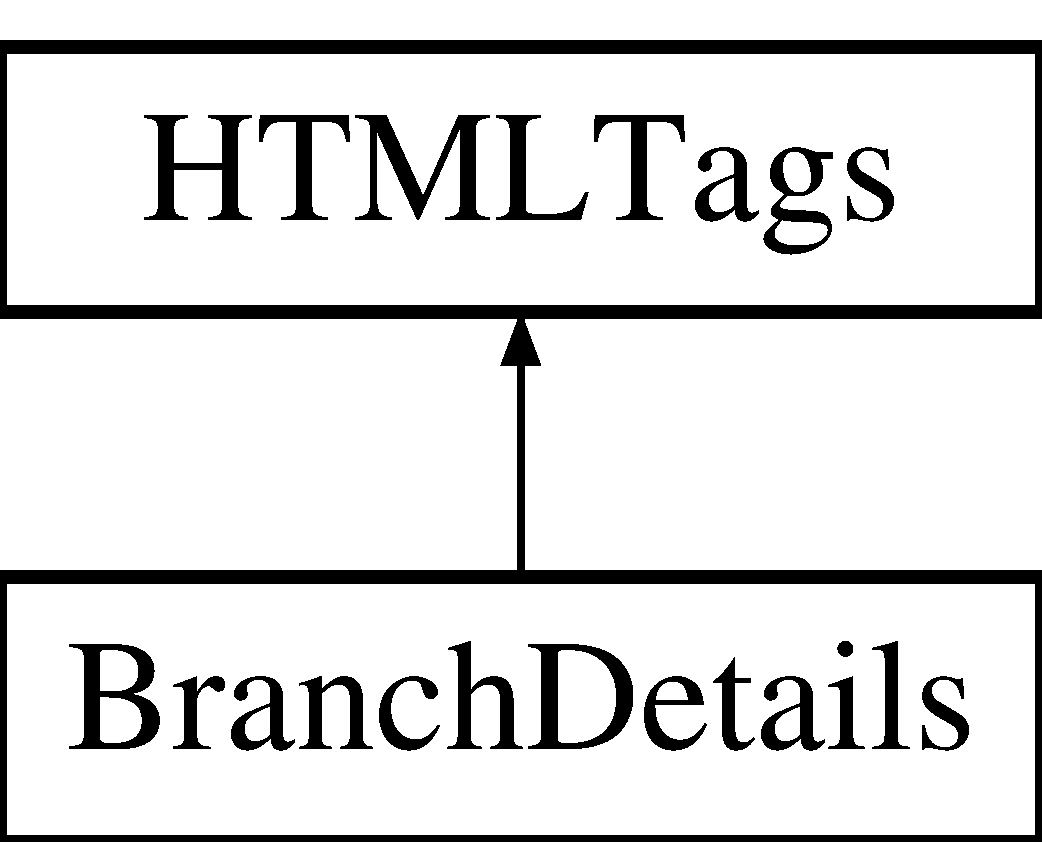
\includegraphics[height=2.000000cm]{classBranchDetails}
\end{center}
\end{figure}
\subsection*{Public Member Functions}
\begin{DoxyCompactItemize}
\item 
\hypertarget{classBranchDetails_a73ad3b9f45e8608a54c68f951149f7b4}{void {\bfseries Head} ()}\label{classBranchDetails_a73ad3b9f45e8608a54c68f951149f7b4}

\item 
\hypertarget{classBranchDetails_a526355c7a1abcd150805d859a6d0d576}{void {\bfseries Javascript} ()}\label{classBranchDetails_a526355c7a1abcd150805d859a6d0d576}

\item 
\hypertarget{classBranchDetails_a4a564cea32737e719441566d284ff849}{void {\bfseries Body} ()}\label{classBranchDetails_a4a564cea32737e719441566d284ff849}

\item 
\hypertarget{classBranchDetails_abfba4740c8618388b79eb6550aad980a}{void {\bfseries Body\-Content} ()}\label{classBranchDetails_abfba4740c8618388b79eb6550aad980a}

\item 
\hypertarget{classBranchDetails_aa44ca0b62d7a37d6723f6135c1672058}{void {\bfseries Main} ()}\label{classBranchDetails_aa44ca0b62d7a37d6723f6135c1672058}

\end{DoxyCompactItemize}
\subsection*{Additional Inherited Members}


The documentation for this class was generated from the following files\-:\begin{DoxyCompactItemize}
\item 
Baka\-Plan/branchdetails.\-h\item 
Baka\-Plan/branchdetails.\-cc\end{DoxyCompactItemize}

\hypertarget{classBranchReport}{\section{Branch\-Report Class Reference}
\label{classBranchReport}\index{Branch\-Report@{Branch\-Report}}
}
Inheritance diagram for Branch\-Report\-:\begin{figure}[H]
\begin{center}
\leavevmode
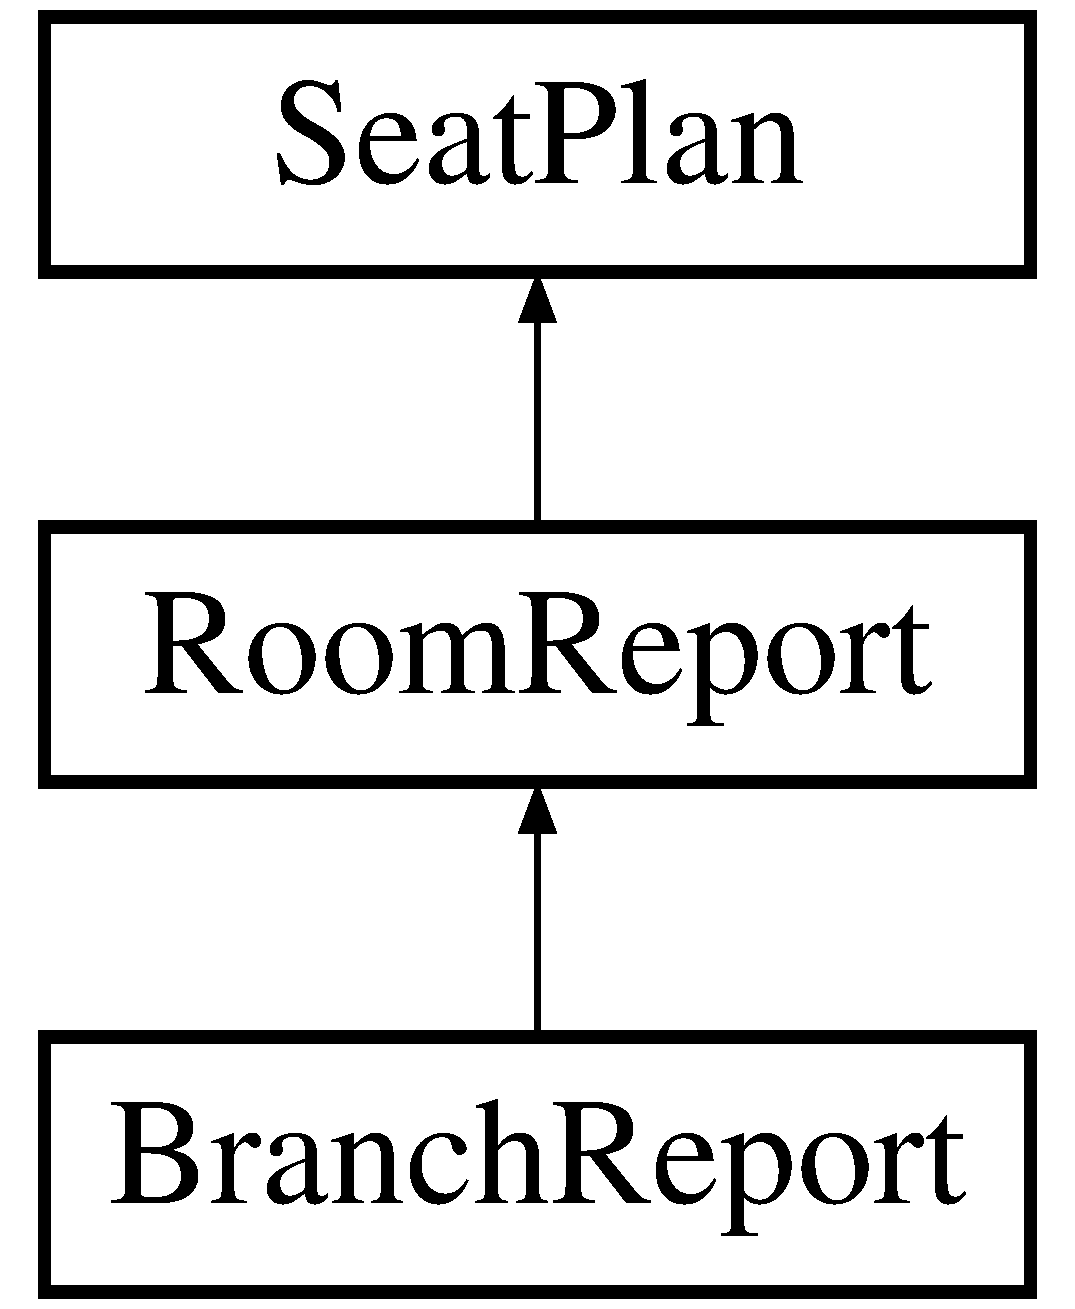
\includegraphics[height=3.000000cm]{classBranchReport}
\end{center}
\end{figure}
\subsection*{Public Member Functions}
\begin{DoxyCompactItemize}
\item 
\hypertarget{classBranchReport_acafa37b5ff6b8886333cc5ab8bb53fad}{void {\bfseries Main} ()}\label{classBranchReport_acafa37b5ff6b8886333cc5ab8bb53fad}

\end{DoxyCompactItemize}
\subsection*{Additional Inherited Members}


The documentation for this class was generated from the following file\-:\begin{DoxyCompactItemize}
\item 
Baka\-Plan/\-Seat\-Plan/report.\-h\end{DoxyCompactItemize}

\hypertarget{classExamDetails}{\section{Exam\-Details Class Reference}
\label{classExamDetails}\index{Exam\-Details@{Exam\-Details}}
}
Inheritance diagram for Exam\-Details\-:\begin{figure}[H]
\begin{center}
\leavevmode
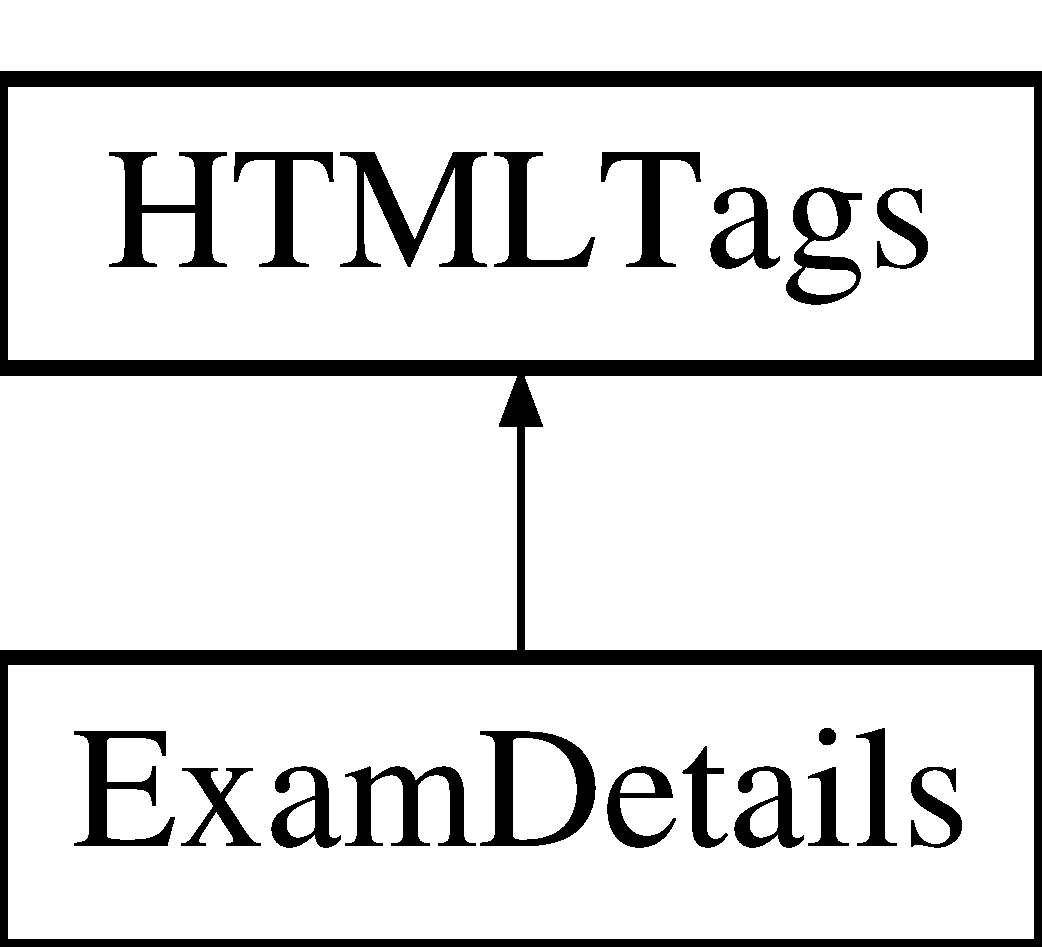
\includegraphics[height=2.000000cm]{classExamDetails}
\end{center}
\end{figure}
\subsection*{Public Member Functions}
\begin{DoxyCompactItemize}
\item 
\hypertarget{classExamDetails_a356f72609abf6d93a6b173af5f28f4db}{void {\bfseries Head} ()}\label{classExamDetails_a356f72609abf6d93a6b173af5f28f4db}

\item 
\hypertarget{classExamDetails_a4925302cb9555f1cadec37872367b0a2}{void {\bfseries Javascript} ()}\label{classExamDetails_a4925302cb9555f1cadec37872367b0a2}

\item 
\hypertarget{classExamDetails_ae8a4c439804372417bcd37976a185626}{void {\bfseries Body} ()}\label{classExamDetails_ae8a4c439804372417bcd37976a185626}

\item 
\hypertarget{classExamDetails_a357e0a4b9116a69af06bd312c809f84e}{void {\bfseries Body\-Content} ()}\label{classExamDetails_a357e0a4b9116a69af06bd312c809f84e}

\item 
\hypertarget{classExamDetails_a9ae3ecade5e455f7b71f4ef46febe71b}{void {\bfseries Main} ()}\label{classExamDetails_a9ae3ecade5e455f7b71f4ef46febe71b}

\end{DoxyCompactItemize}
\subsection*{Additional Inherited Members}


The documentation for this class was generated from the following files\-:\begin{DoxyCompactItemize}
\item 
Baka\-Plan/examdetails.\-h\item 
Baka\-Plan/examdetails.\-cc\end{DoxyCompactItemize}

\hypertarget{classExapandRollNo}{\section{Exapand\-Roll\-No Class Reference}
\label{classExapandRollNo}\index{Exapand\-Roll\-No@{Exapand\-Roll\-No}}
}
Inheritance diagram for Exapand\-Roll\-No\-:\begin{figure}[H]
\begin{center}
\leavevmode
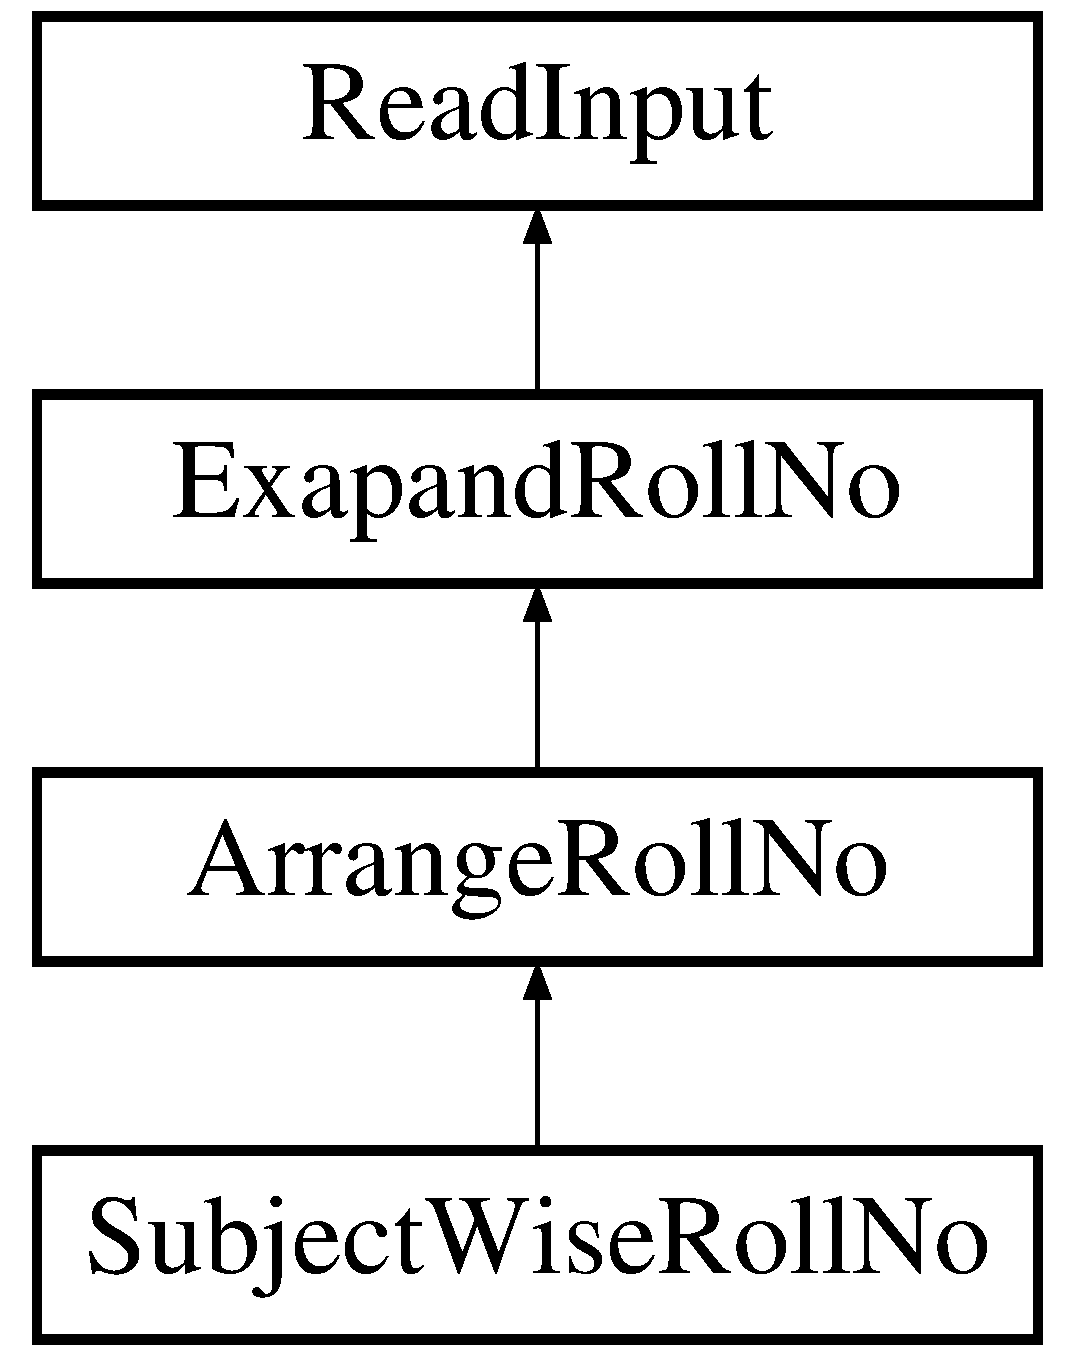
\includegraphics[height=4.000000cm]{classExapandRollNo}
\end{center}
\end{figure}
\subsection*{Public Member Functions}
\begin{DoxyCompactItemize}
\item 
\hypertarget{classExapandRollNo_a19a299d6ebbff3af32fdee08fcc164ee}{void {\bfseries expand\-Input} ()}\label{classExapandRollNo_a19a299d6ebbff3af32fdee08fcc164ee}

\item 
\hypertarget{classExapandRollNo_ad1a2a298aa0834a6da672e152cd4e24f}{void {\bfseries add\-Seperator} ()}\label{classExapandRollNo_ad1a2a298aa0834a6da672e152cd4e24f}

\item 
\hypertarget{classExapandRollNo_a9125b4dc6bbdb81dc4007cec1e86a7e9}{void {\bfseries expand\-Roll\-No} ()}\label{classExapandRollNo_a9125b4dc6bbdb81dc4007cec1e86a7e9}

\item 
\hypertarget{classExapandRollNo_a69ff3dc919a8b297b46926839184b349}{{\footnotesize template$<$typename Out\-Iter $>$ }\\bool {\bfseries expand\-Roll\-Number\-List} (istream \&is, Out\-Iter out)}\label{classExapandRollNo_a69ff3dc919a8b297b46926839184b349}

\item 
\hypertarget{classExapandRollNo_a3b767bfce279771a398abaa725753e33}{void {\bfseries remove\-Zero} ()}\label{classExapandRollNo_a3b767bfce279771a398abaa725753e33}

\item 
\hypertarget{classExapandRollNo_ae11d041a516d6fce629364d6e6796955}{void {\bfseries show\-Expand\-Roll\-No} ()}\label{classExapandRollNo_ae11d041a516d6fce629364d6e6796955}

\item 
\hypertarget{classExapandRollNo_afbfccde139eb71155e0b0fce02962d1c}{void {\bfseries Main} ()}\label{classExapandRollNo_afbfccde139eb71155e0b0fce02962d1c}

\end{DoxyCompactItemize}
\subsection*{Protected Attributes}
\begin{DoxyCompactItemize}
\item 
\hypertarget{classExapandRollNo_ae27a8647cfc7f93a5ba2fbfef8afa5c8}{int {\bfseries roll\-\_\-no} \mbox{[}M\-I\-N\-\_\-\-S\-I\-Z\-E\mbox{]}\mbox{[}M\-A\-X\-\_\-\-S\-I\-Z\-E\mbox{]}\mbox{[}M\-A\-X\-\_\-\-S\-I\-Z\-E\mbox{]}}\label{classExapandRollNo_ae27a8647cfc7f93a5ba2fbfef8afa5c8}

\item 
\hypertarget{classExapandRollNo_a892479a25a021a95e9c4b38ed30208a5}{int {\bfseries roll\-\_\-size} \mbox{[}M\-I\-N\-\_\-\-S\-I\-Z\-E\mbox{]}\mbox{[}M\-I\-N\-\_\-\-S\-I\-Z\-E\mbox{]}}\label{classExapandRollNo_a892479a25a021a95e9c4b38ed30208a5}

\item 
\hypertarget{classExapandRollNo_ac3526c93e25b52ab118f66150c980dbd}{int {\bfseries not\-\_\-roll\-\_\-no} \mbox{[}M\-I\-N\-\_\-\-S\-I\-Z\-E\mbox{]}\mbox{[}M\-A\-X\-\_\-\-S\-I\-Z\-E\mbox{]}\mbox{[}M\-A\-X\-\_\-\-S\-I\-Z\-E\mbox{]}}\label{classExapandRollNo_ac3526c93e25b52ab118f66150c980dbd}

\item 
\hypertarget{classExapandRollNo_a809856dbd610c81509f2fdf2cc11e57f}{int {\bfseries not\-\_\-roll\-\_\-size} \mbox{[}M\-I\-N\-\_\-\-S\-I\-Z\-E\mbox{]}\mbox{[}M\-I\-N\-\_\-\-S\-I\-Z\-E\mbox{]}}\label{classExapandRollNo_a809856dbd610c81509f2fdf2cc11e57f}

\end{DoxyCompactItemize}


The documentation for this class was generated from the following files\-:\begin{DoxyCompactItemize}
\item 
expand-\/rollno.\-h\item 
expand-\/rollno.\-cc\end{DoxyCompactItemize}

\hypertarget{classHome}{\section{Home Class Reference}
\label{classHome}\index{Home@{Home}}
}
Inheritance diagram for Home\-:\begin{figure}[H]
\begin{center}
\leavevmode
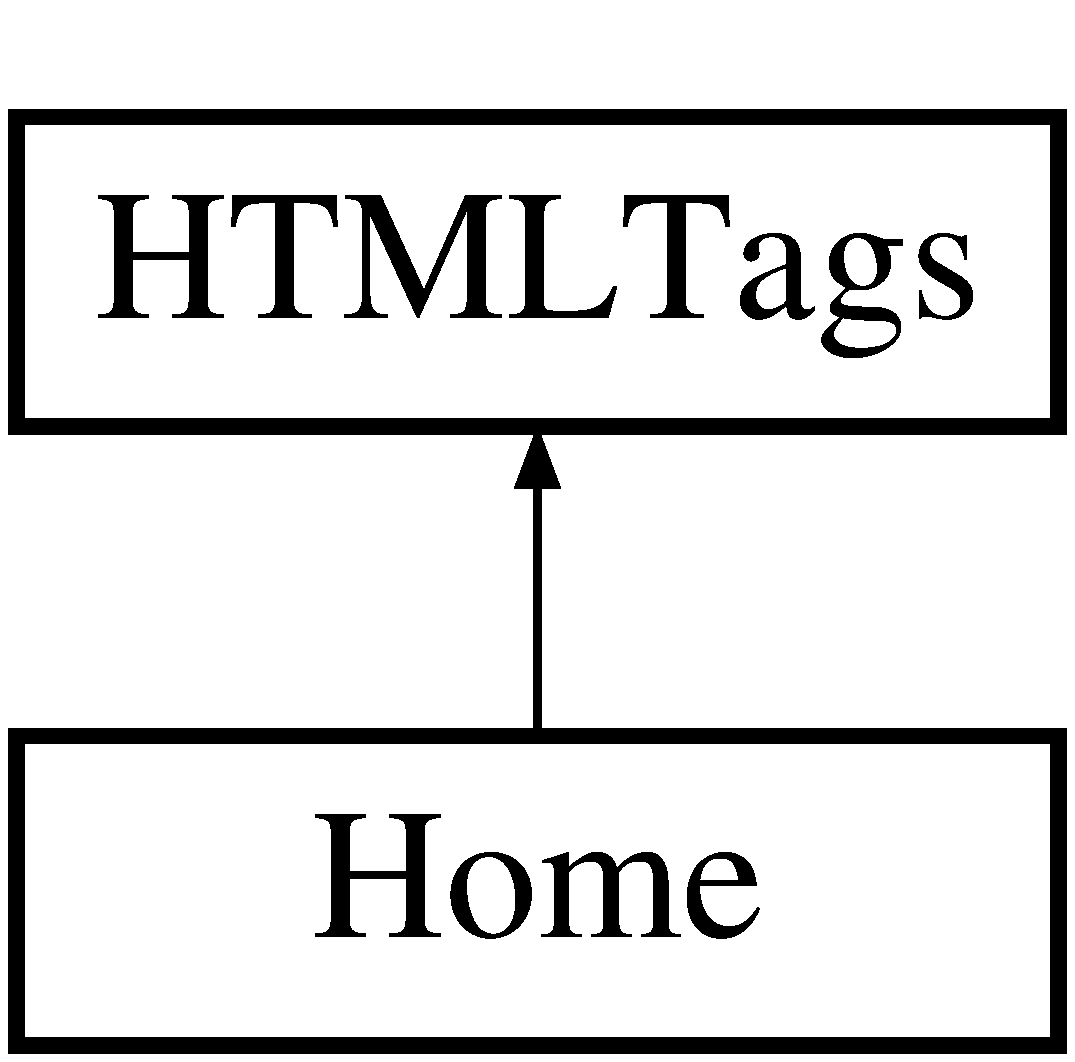
\includegraphics[height=2.000000cm]{classHome}
\end{center}
\end{figure}
\subsection*{Public Member Functions}
\begin{DoxyCompactItemize}
\item 
\hypertarget{classHome_aa327c2af7868c60c181806734e3b00f6}{void {\bfseries Head} ()}\label{classHome_aa327c2af7868c60c181806734e3b00f6}

\item 
\hypertarget{classHome_aa603fee7511d68025346d1e7fed09e80}{void {\bfseries Javascript} ()}\label{classHome_aa603fee7511d68025346d1e7fed09e80}

\item 
\hypertarget{classHome_a008d316a2ff266216dffc74042b6bd25}{void {\bfseries Body} ()}\label{classHome_a008d316a2ff266216dffc74042b6bd25}

\item 
\hypertarget{classHome_ab4cc0a979a58aea15ffdf20517b8f4e4}{void {\bfseries Body\-Content} ()}\label{classHome_ab4cc0a979a58aea15ffdf20517b8f4e4}

\item 
\hypertarget{classHome_aaecd93781c4fa1bd9d7a287c929be2fd}{void {\bfseries Main} ()}\label{classHome_aaecd93781c4fa1bd9d7a287c929be2fd}

\end{DoxyCompactItemize}
\subsection*{Additional Inherited Members}


The documentation for this class was generated from the following files\-:\begin{DoxyCompactItemize}
\item 
Baka\-Plan/home.\-h\item 
Baka\-Plan/home.\-cc\end{DoxyCompactItemize}

\hypertarget{classHomeCSS}{\section{Home\-C\-S\-S Class Reference}
\label{classHomeCSS}\index{Home\-C\-S\-S@{Home\-C\-S\-S}}
}
\subsection*{Public Member Functions}
\begin{DoxyCompactItemize}
\item 
\hypertarget{classHomeCSS_a7b0aa561a4b4aee682b9e51d64db1602}{void {\bfseries Content\-Type} ()}\label{classHomeCSS_a7b0aa561a4b4aee682b9e51d64db1602}

\item 
\hypertarget{classHomeCSS_a6b79a31efcc541dd383218288272d6d6}{void {\bfseries Main} ()}\label{classHomeCSS_a6b79a31efcc541dd383218288272d6d6}

\end{DoxyCompactItemize}


\subsection{Detailed Description}


Definition at line 3 of file css.\-h.



The documentation for this class was generated from the following files\-:\begin{DoxyCompactItemize}
\item 
Baka\-Plan/css.\-h\item 
Baka\-Plan/css.\-cc\end{DoxyCompactItemize}

\hypertarget{classHTMLTags}{\section{H\-T\-M\-L\-Tags Class Reference}
\label{classHTMLTags}\index{H\-T\-M\-L\-Tags@{H\-T\-M\-L\-Tags}}
}


{\ttfamily \#include $<$htmltags.\-h$>$}

Inheritance diagram for H\-T\-M\-L\-Tags\-:\begin{figure}[H]
\begin{center}
\leavevmode
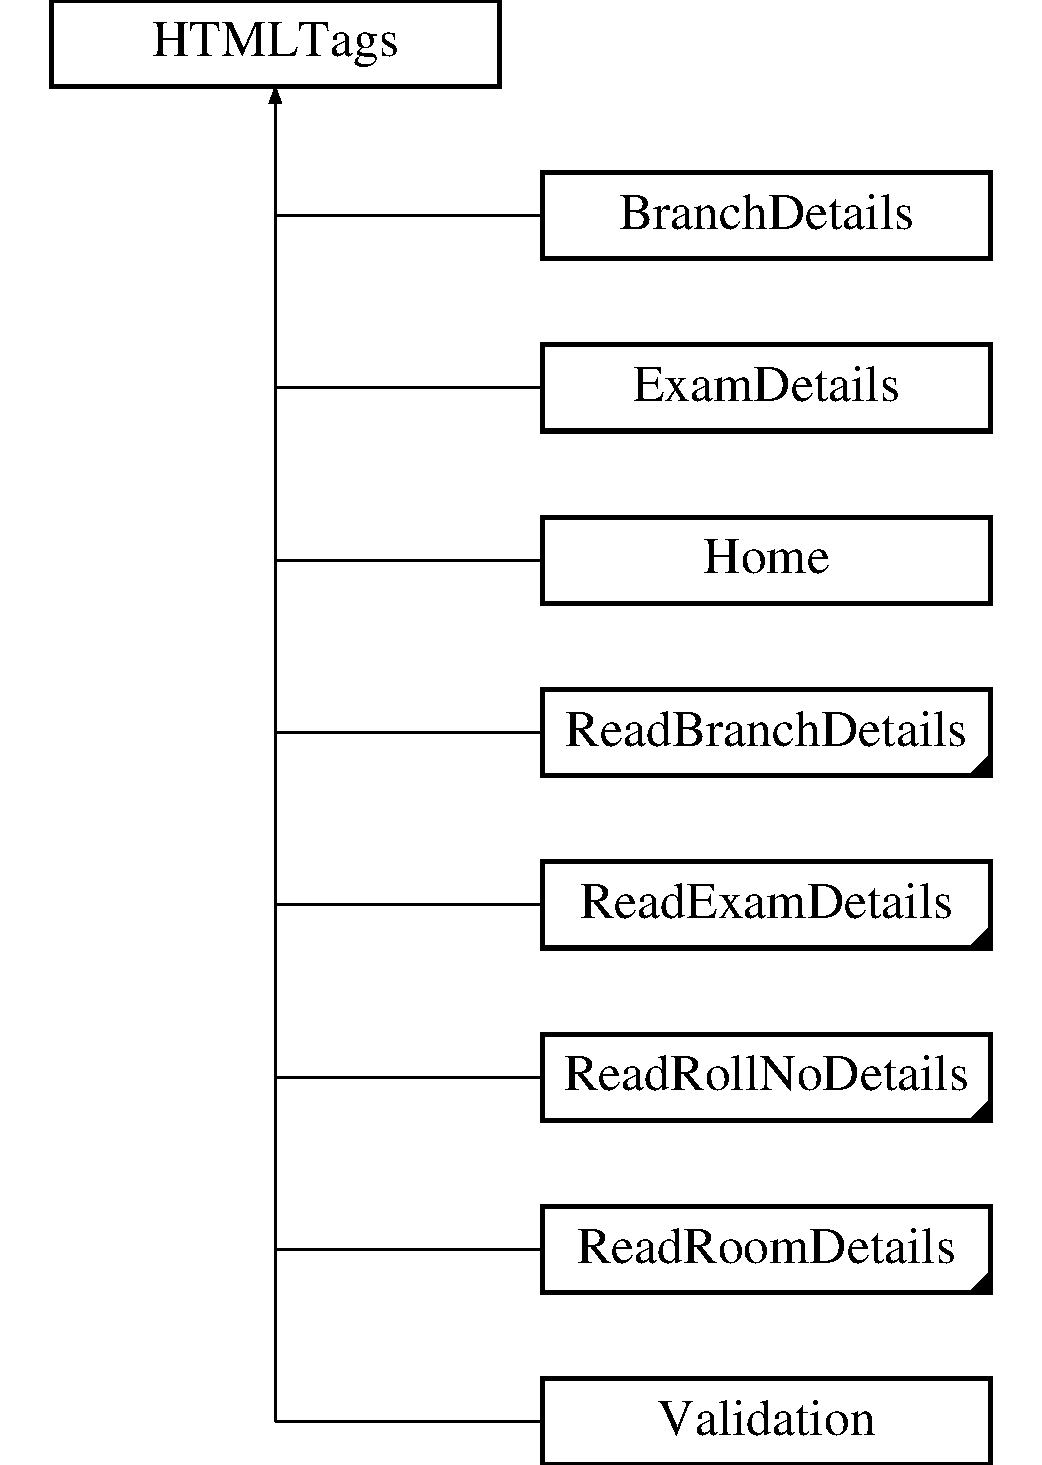
\includegraphics[height=3.000000cm]{classHTMLTags}
\end{center}
\end{figure}
\subsection*{Public Member Functions}
\begin{DoxyCompactItemize}
\item 
\hyperlink{classHTMLTags_a4f0bb4f538b87033b574ff05798eb60b}{H\-T\-M\-L\-Tags} ()
\begin{DoxyCompactList}\small\item\em Constructor. \end{DoxyCompactList}\item 
void \hyperlink{classHTMLTags_abe32ec84b6b2940afbc993be2db178e9}{Set\-H\-T\-M\-L\-Variables} ()
\begin{DoxyCompactList}\small\item\em Assingn Values to variables. \end{DoxyCompactList}\item 
void \hyperlink{classHTMLTags_a567551cd701d2836d4240b2917b5e13f}{H\-T\-M\-L\-Start} ()
\begin{DoxyCompactList}\small\item\em Display $<$\-H\-T\-M\-L$>$ \end{DoxyCompactList}\item 
void \hyperlink{classHTMLTags_a6553c3d01ee194a1d157e6341333dee3}{H\-T\-M\-L\-End} ()
\begin{DoxyCompactList}\small\item\em Display $<$/\-H\-T\-M\-L$>$ \end{DoxyCompactList}\item 
void \hyperlink{classHTMLTags_af2b01cc08884af52e0b291d07035062e}{Head\-Start} ()
\item 
void \hyperlink{classHTMLTags_afdc779e46fac16cc79e4f0e87f621254}{Head\-End} ()
\begin{DoxyCompactList}\small\item\em Display $<$/\-H\-E\-A\-D$>$ \end{DoxyCompactList}\item 
void \hyperlink{classHTMLTags_a5128d6f1c6be5ac1689047fc9d0d159f}{Title} (string page\-Title)
\begin{DoxyCompactList}\small\item\em Display $<$\-T\-I\-T\-L\-E$>$ $<$/\-T\-I\-T\-L\-E$>$ \end{DoxyCompactList}\item 
void \hyperlink{classHTMLTags_a4e9e18580cc7f2b82c82e4f81e39be50}{C\-S\-S} (string href)
\begin{DoxyCompactList}\small\item\em Add External C\-S\-S. \end{DoxyCompactList}\item 
void \hyperlink{classHTMLTags_aea041d720f12a210615c95350774e6aa}{Javascript} (string src)
\begin{DoxyCompactList}\small\item\em Add Javascript File. \end{DoxyCompactList}\item 
void \hyperlink{classHTMLTags_af1fb7b90b9ebb83177da18aba1ef86a9}{Body\-Start} ()
\begin{DoxyCompactList}\small\item\em Display $<$\-B\-O\-D\-Y$>$ \end{DoxyCompactList}\item 
void \hyperlink{classHTMLTags_a7cae36bd3a0e6f35e89494e5cda64971}{Body\-End} ()
\begin{DoxyCompactList}\small\item\em Display $<$/\-B\-O\-D\-Y$>$ \end{DoxyCompactList}\item 
void \hyperlink{classHTMLTags_a897512b202cfd12729e8fa24e67ea4d6}{Div\-Start} (string id, string class\-Name)
\begin{DoxyCompactList}\small\item\em Start Div Section. \end{DoxyCompactList}\item 
void \hyperlink{classHTMLTags_aa82b2d3d85b3afd29e5641dbe1ace439}{Div\-End} ()
\begin{DoxyCompactList}\small\item\em End div section. \end{DoxyCompactList}\item 
void \hyperlink{classHTMLTags_a1489ccf4629069eca5e550eeb8e8e887}{Form\-Start} (string name, string action, string method)
\begin{DoxyCompactList}\small\item\em Start Form. \end{DoxyCompactList}\item 
void \hyperlink{classHTMLTags_ab57baef28db9590ce59d0e2f403a210f}{Form\-End} ()
\begin{DoxyCompactList}\small\item\em End Form. \end{DoxyCompactList}\item 
void \hyperlink{classHTMLTags_a9d4bc37c7d615bc1d7f7c738dae48ad3}{Table\-Start} (string id, string class\-Name)
\begin{DoxyCompactList}\small\item\em Start Table. \end{DoxyCompactList}\item 
void \hyperlink{classHTMLTags_a0655d9f70a8c1a61c406280d8fb9df7a}{Table\-End} ()
\begin{DoxyCompactList}\small\item\em End Table. \end{DoxyCompactList}\item 
void \hyperlink{classHTMLTags_ab515d13346f63b00f7696374e682344e}{Input\-Field} (string type, string name, string value)
\begin{DoxyCompactList}\small\item\em Input Field. \end{DoxyCompactList}\item 
void \hyperlink{classHTMLTags_adb6e7ef0a1320dbf6d4acbe1ea3e418f}{Select\-Field\-Start} (string name)
\begin{DoxyCompactList}\small\item\em Select Field Start. \end{DoxyCompactList}\item 
void \hyperlink{classHTMLTags_adde967a90e03f4b5168b9bffd319980b}{Select\-Field\-End} ()
\begin{DoxyCompactList}\small\item\em End Select Field. \end{DoxyCompactList}\item 
void \hyperlink{classHTMLTags_a09f91c8601aed3aa2d0978123225afaa}{Select\-Option\-Start} (string value)
\begin{DoxyCompactList}\small\item\em Select Option Start. \end{DoxyCompactList}\item 
void \hyperlink{classHTMLTags_ae312980d20e3dea0469fdcb730fb975e}{Select\-Option\-End} ()
\begin{DoxyCompactList}\small\item\em Selct Option End. \end{DoxyCompactList}\item 
void \hyperlink{classHTMLTags_ab6dbb027d808e7b708a4ece7e911ceee}{Button} (string id, string type, string class\-Name, string value)
\begin{DoxyCompactList}\small\item\em Button. \end{DoxyCompactList}\end{DoxyCompactItemize}
\subsection*{Protected Attributes}
\begin{DoxyCompactItemize}
\item 
string \hyperlink{classHTMLTags_ae987289d0dab2e3e234048615f930d0f}{start\-H1}
\begin{DoxyCompactList}\small\item\em H\-T\-M\-L Tag Variables for 

, , 

, etc. \end{DoxyCompactList}\item 
\hypertarget{classHTMLTags_a708194dea85c068a24b7923254fd7458}{string {\bfseries end\-H1}}\label{classHTMLTags_a708194dea85c068a24b7923254fd7458}

\item 
\hypertarget{classHTMLTags_a9290221d987dfe55acd3d2002a48efa0}{string {\bfseries start\-H3}}\label{classHTMLTags_a9290221d987dfe55acd3d2002a48efa0}

\item 
\hypertarget{classHTMLTags_afa471891c94946ba4a68acd727246d66}{string {\bfseries end\-H3}}\label{classHTMLTags_afa471891c94946ba4a68acd727246d66}

\item 
\hypertarget{classHTMLTags_a827d77a9a5cc3c442421420f0713c17a}{string {\bfseries start\-T\-D}}\label{classHTMLTags_a827d77a9a5cc3c442421420f0713c17a}

\item 
\hypertarget{classHTMLTags_ac2f4aae38f9d88d90df443e1e59a5bfc}{string {\bfseries end\-T\-D}}\label{classHTMLTags_ac2f4aae38f9d88d90df443e1e59a5bfc}

\item 
\hypertarget{classHTMLTags_a71b8a6e9593c6744f75fe8fac83e39b7}{string {\bfseries start\-T\-H}}\label{classHTMLTags_a71b8a6e9593c6744f75fe8fac83e39b7}

\item 
\hypertarget{classHTMLTags_a12cc718fee6ac4d701aafa9bc6303ad3}{string {\bfseries end\-T\-H}}\label{classHTMLTags_a12cc718fee6ac4d701aafa9bc6303ad3}

\item 
\hypertarget{classHTMLTags_ae8ee5ce9589d18b36263d62c6aa30e0a}{string {\bfseries start\-T\-R}}\label{classHTMLTags_ae8ee5ce9589d18b36263d62c6aa30e0a}

\item 
\hypertarget{classHTMLTags_ae6b79efff5ed7c253a050a6179057942}{string {\bfseries end\-T\-R}}\label{classHTMLTags_ae6b79efff5ed7c253a050a6179057942}

\item 
\hypertarget{classHTMLTags_ac6dafb63a2da3f7500cc080fd43a324d}{string {\bfseries start\-B}}\label{classHTMLTags_ac6dafb63a2da3f7500cc080fd43a324d}

\item 
\hypertarget{classHTMLTags_a12fc9d60d71c585cfba1643dc93eb8fc}{string {\bfseries end\-B}}\label{classHTMLTags_a12fc9d60d71c585cfba1643dc93eb8fc}

\end{DoxyCompactItemize}


\subsection{Detailed Description}
\subsection*{Include Header file }

Class\-: \hyperlink{classHTMLTags}{H\-T\-M\-L\-Tags} \subsection*{Description\-: Declaration}

Definition at line 30 of file htmltags.\-h.



\subsection{Constructor \& Destructor Documentation}
\hypertarget{classHTMLTags_a4f0bb4f538b87033b574ff05798eb60b}{\index{H\-T\-M\-L\-Tags@{H\-T\-M\-L\-Tags}!H\-T\-M\-L\-Tags@{H\-T\-M\-L\-Tags}}
\index{H\-T\-M\-L\-Tags@{H\-T\-M\-L\-Tags}!HTMLTags@{H\-T\-M\-L\-Tags}}
\subsubsection[{H\-T\-M\-L\-Tags}]{\setlength{\rightskip}{0pt plus 5cm}H\-T\-M\-L\-Tags\-::\-H\-T\-M\-L\-Tags (
\begin{DoxyParamCaption}
{}
\end{DoxyParamCaption}
)}}\label{classHTMLTags_a4f0bb4f538b87033b574ff05798eb60b}


Constructor. 



 Class\-: \hyperlink{classHTMLTags}{H\-T\-M\-L\-Tags} Method\-: \hyperlink{classHTMLTags}{H\-T\-M\-L\-Tags} \-:\-: \hyperlink{classHTMLTags_a4f0bb4f538b87033b574ff05798eb60b}{H\-T\-M\-L\-Tags()} \subsubsection*{Description\-: Constructor}

Definition at line 27 of file htmltags.\-cc.



\subsection{Member Function Documentation}
\hypertarget{classHTMLTags_a7cae36bd3a0e6f35e89494e5cda64971}{\index{H\-T\-M\-L\-Tags@{H\-T\-M\-L\-Tags}!Body\-End@{Body\-End}}
\index{Body\-End@{Body\-End}!HTMLTags@{H\-T\-M\-L\-Tags}}
\subsubsection[{Body\-End}]{\setlength{\rightskip}{0pt plus 5cm}void H\-T\-M\-L\-Tags\-::\-Body\-End (
\begin{DoxyParamCaption}
{}
\end{DoxyParamCaption}
)}}\label{classHTMLTags_a7cae36bd3a0e6f35e89494e5cda64971}


Display $<$/\-B\-O\-D\-Y$>$ 



 Class\-: \hyperlink{classHTMLTags}{H\-T\-M\-L\-Tags} Method\-: \hyperlink{classHTMLTags}{H\-T\-M\-L\-Tags} \-:\-: \hyperlink{classHTMLTags_a7cae36bd3a0e6f35e89494e5cda64971}{Body\-End()} \subsubsection*{Description\-: Display }

Definition at line 172 of file htmltags.\-cc.

\hypertarget{classHTMLTags_af1fb7b90b9ebb83177da18aba1ef86a9}{\index{H\-T\-M\-L\-Tags@{H\-T\-M\-L\-Tags}!Body\-Start@{Body\-Start}}
\index{Body\-Start@{Body\-Start}!HTMLTags@{H\-T\-M\-L\-Tags}}
\subsubsection[{Body\-Start}]{\setlength{\rightskip}{0pt plus 5cm}void H\-T\-M\-L\-Tags\-::\-Body\-Start (
\begin{DoxyParamCaption}
{}
\end{DoxyParamCaption}
)}}\label{classHTMLTags_af1fb7b90b9ebb83177da18aba1ef86a9}


Display $<$\-B\-O\-D\-Y$>$ 



 Class\-: \hyperlink{classHTMLTags}{H\-T\-M\-L\-Tags} Method\-: \hyperlink{classHTMLTags}{H\-T\-M\-L\-Tags} \-:\-: \hyperlink{classHTMLTags_af1fb7b90b9ebb83177da18aba1ef86a9}{Body\-Start()} \subsubsection*{Description\-: Display }

Definition at line 159 of file htmltags.\-cc.

\hypertarget{classHTMLTags_ab6dbb027d808e7b708a4ece7e911ceee}{\index{H\-T\-M\-L\-Tags@{H\-T\-M\-L\-Tags}!Button@{Button}}
\index{Button@{Button}!HTMLTags@{H\-T\-M\-L\-Tags}}
\subsubsection[{Button}]{\setlength{\rightskip}{0pt plus 5cm}void H\-T\-M\-L\-Tags\-::\-Button (
\begin{DoxyParamCaption}
\item[{string}]{id, }
\item[{string}]{type, }
\item[{string}]{class\-Name, }
\item[{string}]{value}
\end{DoxyParamCaption}
)}}\label{classHTMLTags_ab6dbb027d808e7b708a4ece7e911ceee}


Button. 



 Class\-: \hyperlink{classHTMLTags}{H\-T\-M\-L\-Tags} Method\-: \hyperlink{classHTMLTags}{H\-T\-M\-L\-Tags} \-:\-: Button(string id, string type, string class\-Name, string value) \subsubsection*{Description\-: Create button(next, submit, etc)}

Definition at line 340 of file htmltags.\-cc.

\hypertarget{classHTMLTags_a4e9e18580cc7f2b82c82e4f81e39be50}{\index{H\-T\-M\-L\-Tags@{H\-T\-M\-L\-Tags}!C\-S\-S@{C\-S\-S}}
\index{C\-S\-S@{C\-S\-S}!HTMLTags@{H\-T\-M\-L\-Tags}}
\subsubsection[{C\-S\-S}]{\setlength{\rightskip}{0pt plus 5cm}void H\-T\-M\-L\-Tags\-::\-C\-S\-S (
\begin{DoxyParamCaption}
\item[{string}]{href}
\end{DoxyParamCaption}
)}}\label{classHTMLTags_a4e9e18580cc7f2b82c82e4f81e39be50}


Add External C\-S\-S. 



 Class\-: \hyperlink{classHTMLTags}{H\-T\-M\-L\-Tags} Method\-: \hyperlink{classHTMLTags}{H\-T\-M\-L\-Tags} \-:\-: \hyperlink{classHTMLTags_a4e9e18580cc7f2b82c82e4f81e39be50}{C\-S\-S(string href)} \subsubsection*{Description\-: Add External C\-S\-S file}

Definition at line 131 of file htmltags.\-cc.

\hypertarget{classHTMLTags_aa82b2d3d85b3afd29e5641dbe1ace439}{\index{H\-T\-M\-L\-Tags@{H\-T\-M\-L\-Tags}!Div\-End@{Div\-End}}
\index{Div\-End@{Div\-End}!HTMLTags@{H\-T\-M\-L\-Tags}}
\subsubsection[{Div\-End}]{\setlength{\rightskip}{0pt plus 5cm}void H\-T\-M\-L\-Tags\-::\-Div\-End (
\begin{DoxyParamCaption}
{}
\end{DoxyParamCaption}
)}}\label{classHTMLTags_aa82b2d3d85b3afd29e5641dbe1ace439}


End div section. 



 Class\-: \hyperlink{classHTMLTags}{H\-T\-M\-L\-Tags} Method\-: \hyperlink{classHTMLTags}{H\-T\-M\-L\-Tags} \-:\-: \hyperlink{classHTMLTags_aa82b2d3d85b3afd29e5641dbe1ace439}{Div\-End()} \subsubsection*{Description\-: Close Div Section}

Definition at line 199 of file htmltags.\-cc.

\hypertarget{classHTMLTags_a897512b202cfd12729e8fa24e67ea4d6}{\index{H\-T\-M\-L\-Tags@{H\-T\-M\-L\-Tags}!Div\-Start@{Div\-Start}}
\index{Div\-Start@{Div\-Start}!HTMLTags@{H\-T\-M\-L\-Tags}}
\subsubsection[{Div\-Start}]{\setlength{\rightskip}{0pt plus 5cm}void H\-T\-M\-L\-Tags\-::\-Div\-Start (
\begin{DoxyParamCaption}
\item[{string}]{id, }
\item[{string}]{class\-Name}
\end{DoxyParamCaption}
)}}\label{classHTMLTags_a897512b202cfd12729e8fa24e67ea4d6}


Start Div Section. 



 Class\-: \hyperlink{classHTMLTags}{H\-T\-M\-L\-Tags} Method\-: \hyperlink{classHTMLTags}{H\-T\-M\-L\-Tags} \-:\-: \hyperlink{classHTMLTags_a897512b202cfd12729e8fa24e67ea4d6}{Div\-Start(string id, string class\-Name)} \subsubsection*{Description\-: Start Div Section with id and class\-Name(for C\-S\-S)}

Definition at line 185 of file htmltags.\-cc.

\hypertarget{classHTMLTags_ab57baef28db9590ce59d0e2f403a210f}{\index{H\-T\-M\-L\-Tags@{H\-T\-M\-L\-Tags}!Form\-End@{Form\-End}}
\index{Form\-End@{Form\-End}!HTMLTags@{H\-T\-M\-L\-Tags}}
\subsubsection[{Form\-End}]{\setlength{\rightskip}{0pt plus 5cm}void H\-T\-M\-L\-Tags\-::\-Form\-End (
\begin{DoxyParamCaption}
{}
\end{DoxyParamCaption}
)}}\label{classHTMLTags_ab57baef28db9590ce59d0e2f403a210f}


End Form. 



 Class\-: \hyperlink{classHTMLTags}{H\-T\-M\-L\-Tags} Method\-: \hyperlink{classHTMLTags}{H\-T\-M\-L\-Tags} \-:\-: \hyperlink{classHTMLTags_ab57baef28db9590ce59d0e2f403a210f}{Form\-End()} \subsubsection*{Description\-: Close Form}

Definition at line 227 of file htmltags.\-cc.

\hypertarget{classHTMLTags_a1489ccf4629069eca5e550eeb8e8e887}{\index{H\-T\-M\-L\-Tags@{H\-T\-M\-L\-Tags}!Form\-Start@{Form\-Start}}
\index{Form\-Start@{Form\-Start}!HTMLTags@{H\-T\-M\-L\-Tags}}
\subsubsection[{Form\-Start}]{\setlength{\rightskip}{0pt plus 5cm}void H\-T\-M\-L\-Tags\-::\-Form\-Start (
\begin{DoxyParamCaption}
\item[{string}]{name, }
\item[{string}]{action, }
\item[{string}]{method}
\end{DoxyParamCaption}
)}}\label{classHTMLTags_a1489ccf4629069eca5e550eeb8e8e887}


Start Form. 



 Class\-: \hyperlink{classHTMLTags}{H\-T\-M\-L\-Tags} Method\-: \hyperlink{classHTMLTags}{H\-T\-M\-L\-Tags} \-:\-: Form\-Start(string name, string action, string method) \subsubsection*{Description\-: Start Form with name, action and method(G\-E\-T/\-P\-O\-S\-T)}

Definition at line 213 of file htmltags.\-cc.

\hypertarget{classHTMLTags_afdc779e46fac16cc79e4f0e87f621254}{\index{H\-T\-M\-L\-Tags@{H\-T\-M\-L\-Tags}!Head\-End@{Head\-End}}
\index{Head\-End@{Head\-End}!HTMLTags@{H\-T\-M\-L\-Tags}}
\subsubsection[{Head\-End}]{\setlength{\rightskip}{0pt plus 5cm}void H\-T\-M\-L\-Tags\-::\-Head\-End (
\begin{DoxyParamCaption}
{}
\end{DoxyParamCaption}
)}}\label{classHTMLTags_afdc779e46fac16cc79e4f0e87f621254}


Display $<$/\-H\-E\-A\-D$>$ 



 Class\-: \hyperlink{classHTMLTags}{H\-T\-M\-L\-Tags} Method\-: \hyperlink{classHTMLTags}{H\-T\-M\-L\-Tags} \-:\-: \hyperlink{classHTMLTags_afdc779e46fac16cc79e4f0e87f621254}{Head\-End()} \subsubsection*{Description\-: Display }

Definition at line 105 of file htmltags.\-cc.

\hypertarget{classHTMLTags_af2b01cc08884af52e0b291d07035062e}{\index{H\-T\-M\-L\-Tags@{H\-T\-M\-L\-Tags}!Head\-Start@{Head\-Start}}
\index{Head\-Start@{Head\-Start}!HTMLTags@{H\-T\-M\-L\-Tags}}
\subsubsection[{Head\-Start}]{\setlength{\rightskip}{0pt plus 5cm}void H\-T\-M\-L\-Tags\-::\-Head\-Start (
\begin{DoxyParamCaption}
{}
\end{DoxyParamCaption}
)}}\label{classHTMLTags_af2b01cc08884af52e0b291d07035062e}


 Class\-: \hyperlink{classHTMLTags}{H\-T\-M\-L\-Tags} Method\-: \hyperlink{classHTMLTags}{H\-T\-M\-L\-Tags} \-:\-: \hyperlink{classHTMLTags_af2b01cc08884af52e0b291d07035062e}{Head\-Start()} \subsubsection*{Description\-: Display }

Definition at line 92 of file htmltags.\-cc.

\hypertarget{classHTMLTags_a6553c3d01ee194a1d157e6341333dee3}{\index{H\-T\-M\-L\-Tags@{H\-T\-M\-L\-Tags}!H\-T\-M\-L\-End@{H\-T\-M\-L\-End}}
\index{H\-T\-M\-L\-End@{H\-T\-M\-L\-End}!HTMLTags@{H\-T\-M\-L\-Tags}}
\subsubsection[{H\-T\-M\-L\-End}]{\setlength{\rightskip}{0pt plus 5cm}void H\-T\-M\-L\-Tags\-::\-H\-T\-M\-L\-End (
\begin{DoxyParamCaption}
{}
\end{DoxyParamCaption}
)}}\label{classHTMLTags_a6553c3d01ee194a1d157e6341333dee3}


Display $<$/\-H\-T\-M\-L$>$ 



 Class\-: \hyperlink{classHTMLTags}{H\-T\-M\-L\-Tags} Method\-: \hyperlink{classHTMLTags}{H\-T\-M\-L\-Tags} \-:\-: \hyperlink{classHTMLTags_a6553c3d01ee194a1d157e6341333dee3}{H\-T\-M\-L\-End()} \subsubsection*{Description\-: Display }

Definition at line 79 of file htmltags.\-cc.

\hypertarget{classHTMLTags_a567551cd701d2836d4240b2917b5e13f}{\index{H\-T\-M\-L\-Tags@{H\-T\-M\-L\-Tags}!H\-T\-M\-L\-Start@{H\-T\-M\-L\-Start}}
\index{H\-T\-M\-L\-Start@{H\-T\-M\-L\-Start}!HTMLTags@{H\-T\-M\-L\-Tags}}
\subsubsection[{H\-T\-M\-L\-Start}]{\setlength{\rightskip}{0pt plus 5cm}void H\-T\-M\-L\-Tags\-::\-H\-T\-M\-L\-Start (
\begin{DoxyParamCaption}
{}
\end{DoxyParamCaption}
)}}\label{classHTMLTags_a567551cd701d2836d4240b2917b5e13f}


Display $<$\-H\-T\-M\-L$>$ 



 Class\-: \hyperlink{classHTMLTags}{H\-T\-M\-L\-Tags} Method\-: \hyperlink{classHTMLTags}{H\-T\-M\-L\-Tags} \-:\-: \hyperlink{classHTMLTags_a567551cd701d2836d4240b2917b5e13f}{H\-T\-M\-L\-Start()} \subsubsection*{Description\-: Display  Tag }

Definition at line 66 of file htmltags.\-cc.

\hypertarget{classHTMLTags_ab515d13346f63b00f7696374e682344e}{\index{H\-T\-M\-L\-Tags@{H\-T\-M\-L\-Tags}!Input\-Field@{Input\-Field}}
\index{Input\-Field@{Input\-Field}!HTMLTags@{H\-T\-M\-L\-Tags}}
\subsubsection[{Input\-Field}]{\setlength{\rightskip}{0pt plus 5cm}void H\-T\-M\-L\-Tags\-::\-Input\-Field (
\begin{DoxyParamCaption}
\item[{string}]{type, }
\item[{string}]{name, }
\item[{string}]{value}
\end{DoxyParamCaption}
)}}\label{classHTMLTags_ab515d13346f63b00f7696374e682344e}


Input Field. 



 Class\-: \hyperlink{classHTMLTags}{H\-T\-M\-L\-Tags} Method\-: \hyperlink{classHTMLTags}{H\-T\-M\-L\-Tags} \-:\-: Input\-Field(string type, string name, string value) Description\-: Create Input fields like text field, submit \subsubsection*{button, etc.}

Definition at line 269 of file htmltags.\-cc.

\hypertarget{classHTMLTags_aea041d720f12a210615c95350774e6aa}{\index{H\-T\-M\-L\-Tags@{H\-T\-M\-L\-Tags}!Javascript@{Javascript}}
\index{Javascript@{Javascript}!HTMLTags@{H\-T\-M\-L\-Tags}}
\subsubsection[{Javascript}]{\setlength{\rightskip}{0pt plus 5cm}void H\-T\-M\-L\-Tags\-::\-Javascript (
\begin{DoxyParamCaption}
\item[{string}]{src}
\end{DoxyParamCaption}
)}}\label{classHTMLTags_aea041d720f12a210615c95350774e6aa}


Add Javascript File. 



 Class\-: \hyperlink{classHTMLTags}{H\-T\-M\-L\-Tags} Method\-: \hyperlink{classHTMLTags}{H\-T\-M\-L\-Tags} \-:\-: \hyperlink{classHTMLTags_aea041d720f12a210615c95350774e6aa}{Javascript(string src)} \subsubsection*{Description\-: Add external Javascript file}

Definition at line 146 of file htmltags.\-cc.

\hypertarget{classHTMLTags_adde967a90e03f4b5168b9bffd319980b}{\index{H\-T\-M\-L\-Tags@{H\-T\-M\-L\-Tags}!Select\-Field\-End@{Select\-Field\-End}}
\index{Select\-Field\-End@{Select\-Field\-End}!HTMLTags@{H\-T\-M\-L\-Tags}}
\subsubsection[{Select\-Field\-End}]{\setlength{\rightskip}{0pt plus 5cm}void H\-T\-M\-L\-Tags\-::\-Select\-Field\-End (
\begin{DoxyParamCaption}
{}
\end{DoxyParamCaption}
)}}\label{classHTMLTags_adde967a90e03f4b5168b9bffd319980b}


End Select Field. 



 Class\-: \hyperlink{classHTMLTags}{H\-T\-M\-L\-Tags} Method\-: \hyperlink{classHTMLTags}{H\-T\-M\-L\-Tags} \-:\-: \hyperlink{classHTMLTags_adde967a90e03f4b5168b9bffd319980b}{Select\-Field\-End()} \subsubsection*{Description\-: Close select field}

Definition at line 296 of file htmltags.\-cc.

\hypertarget{classHTMLTags_adb6e7ef0a1320dbf6d4acbe1ea3e418f}{\index{H\-T\-M\-L\-Tags@{H\-T\-M\-L\-Tags}!Select\-Field\-Start@{Select\-Field\-Start}}
\index{Select\-Field\-Start@{Select\-Field\-Start}!HTMLTags@{H\-T\-M\-L\-Tags}}
\subsubsection[{Select\-Field\-Start}]{\setlength{\rightskip}{0pt plus 5cm}void H\-T\-M\-L\-Tags\-::\-Select\-Field\-Start (
\begin{DoxyParamCaption}
\item[{string}]{name}
\end{DoxyParamCaption}
)}}\label{classHTMLTags_adb6e7ef0a1320dbf6d4acbe1ea3e418f}


Select Field Start. 



 Class\-: \hyperlink{classHTMLTags}{H\-T\-M\-L\-Tags} Method\-: \hyperlink{classHTMLTags}{H\-T\-M\-L\-Tags} \-:\-: \hyperlink{classHTMLTags_adb6e7ef0a1320dbf6d4acbe1ea3e418f}{Select\-Field\-Start(string name)} \subsubsection*{Description\-: Create Select Field}

Definition at line 283 of file htmltags.\-cc.

\hypertarget{classHTMLTags_ae312980d20e3dea0469fdcb730fb975e}{\index{H\-T\-M\-L\-Tags@{H\-T\-M\-L\-Tags}!Select\-Option\-End@{Select\-Option\-End}}
\index{Select\-Option\-End@{Select\-Option\-End}!HTMLTags@{H\-T\-M\-L\-Tags}}
\subsubsection[{Select\-Option\-End}]{\setlength{\rightskip}{0pt plus 5cm}void H\-T\-M\-L\-Tags\-::\-Select\-Option\-End (
\begin{DoxyParamCaption}
{}
\end{DoxyParamCaption}
)}}\label{classHTMLTags_ae312980d20e3dea0469fdcb730fb975e}


Selct Option End. 



 Class\-: \hyperlink{classHTMLTags}{H\-T\-M\-L\-Tags} Method\-: \hyperlink{classHTMLTags}{H\-T\-M\-L\-Tags} \-:\-: \hyperlink{classHTMLTags_ae312980d20e3dea0469fdcb730fb975e}{Select\-Option\-End()} \subsubsection*{Description\-: Close select option}

Definition at line 326 of file htmltags.\-cc.

\hypertarget{classHTMLTags_a09f91c8601aed3aa2d0978123225afaa}{\index{H\-T\-M\-L\-Tags@{H\-T\-M\-L\-Tags}!Select\-Option\-Start@{Select\-Option\-Start}}
\index{Select\-Option\-Start@{Select\-Option\-Start}!HTMLTags@{H\-T\-M\-L\-Tags}}
\subsubsection[{Select\-Option\-Start}]{\setlength{\rightskip}{0pt plus 5cm}void H\-T\-M\-L\-Tags\-::\-Select\-Option\-Start (
\begin{DoxyParamCaption}
\item[{string}]{value}
\end{DoxyParamCaption}
)}}\label{classHTMLTags_a09f91c8601aed3aa2d0978123225afaa}


Select Option Start. 



 Class\-: \hyperlink{classHTMLTags}{H\-T\-M\-L\-Tags} Method\-: \hyperlink{classHTMLTags}{H\-T\-M\-L\-Tags} \-:\-: Select\-Option\-Start(string value, string selected) \subsubsection*{Description\-: Options for select }

Definition at line 310 of file htmltags.\-cc.

\hypertarget{classHTMLTags_abe32ec84b6b2940afbc993be2db178e9}{\index{H\-T\-M\-L\-Tags@{H\-T\-M\-L\-Tags}!Set\-H\-T\-M\-L\-Variables@{Set\-H\-T\-M\-L\-Variables}}
\index{Set\-H\-T\-M\-L\-Variables@{Set\-H\-T\-M\-L\-Variables}!HTMLTags@{H\-T\-M\-L\-Tags}}
\subsubsection[{Set\-H\-T\-M\-L\-Variables}]{\setlength{\rightskip}{0pt plus 5cm}void H\-T\-M\-L\-Tags\-::\-Set\-H\-T\-M\-L\-Variables (
\begin{DoxyParamCaption}
{}
\end{DoxyParamCaption}
)}}\label{classHTMLTags_abe32ec84b6b2940afbc993be2db178e9}


Assingn Values to variables. 



 Class\-: \hyperlink{classHTMLTags}{H\-T\-M\-L\-Tags} Method\-: \hyperlink{classHTMLTags}{H\-T\-M\-L\-Tags} \-:\-: \hyperlink{classHTMLTags_abe32ec84b6b2940afbc993be2db178e9}{Set\-H\-T\-M\-L\-Variables()} Description\-: Set values of common H\-T\-M\-L tags in respective \subsubsection*{variables.}

Definition at line 42 of file htmltags.\-cc.

\hypertarget{classHTMLTags_a0655d9f70a8c1a61c406280d8fb9df7a}{\index{H\-T\-M\-L\-Tags@{H\-T\-M\-L\-Tags}!Table\-End@{Table\-End}}
\index{Table\-End@{Table\-End}!HTMLTags@{H\-T\-M\-L\-Tags}}
\subsubsection[{Table\-End}]{\setlength{\rightskip}{0pt plus 5cm}void H\-T\-M\-L\-Tags\-::\-Table\-End (
\begin{DoxyParamCaption}
{}
\end{DoxyParamCaption}
)}}\label{classHTMLTags_a0655d9f70a8c1a61c406280d8fb9df7a}


End Table. 



 Class\-: \hyperlink{classHTMLTags}{H\-T\-M\-L\-Tags} Method\-: \hyperlink{classHTMLTags}{H\-T\-M\-L\-Tags} \-:\-: \hyperlink{classHTMLTags_a0655d9f70a8c1a61c406280d8fb9df7a}{Table\-End()} \subsubsection*{Description\-: Close Table tag}

Definition at line 254 of file htmltags.\-cc.

\hypertarget{classHTMLTags_a9d4bc37c7d615bc1d7f7c738dae48ad3}{\index{H\-T\-M\-L\-Tags@{H\-T\-M\-L\-Tags}!Table\-Start@{Table\-Start}}
\index{Table\-Start@{Table\-Start}!HTMLTags@{H\-T\-M\-L\-Tags}}
\subsubsection[{Table\-Start}]{\setlength{\rightskip}{0pt plus 5cm}void H\-T\-M\-L\-Tags\-::\-Table\-Start (
\begin{DoxyParamCaption}
\item[{string}]{id, }
\item[{string}]{class\-Name}
\end{DoxyParamCaption}
)}}\label{classHTMLTags_a9d4bc37c7d615bc1d7f7c738dae48ad3}


Start Table. 



 Class\-: \hyperlink{classHTMLTags}{H\-T\-M\-L\-Tags} Method\-: \hyperlink{classHTMLTags}{H\-T\-M\-L\-Tags} \-:\-: \hyperlink{classHTMLTags_a9d4bc37c7d615bc1d7f7c738dae48ad3}{Table\-Start(string id, string class\-Name)} \subsubsection*{Description\-: Start Table with id and class\-Name(\-C\-S\-S) attributes}

Definition at line 240 of file htmltags.\-cc.

\hypertarget{classHTMLTags_a5128d6f1c6be5ac1689047fc9d0d159f}{\index{H\-T\-M\-L\-Tags@{H\-T\-M\-L\-Tags}!Title@{Title}}
\index{Title@{Title}!HTMLTags@{H\-T\-M\-L\-Tags}}
\subsubsection[{Title}]{\setlength{\rightskip}{0pt plus 5cm}void H\-T\-M\-L\-Tags\-::\-Title (
\begin{DoxyParamCaption}
\item[{string}]{page\-Title}
\end{DoxyParamCaption}
)}}\label{classHTMLTags_a5128d6f1c6be5ac1689047fc9d0d159f}


Display $<$\-T\-I\-T\-L\-E$>$ $<$/\-T\-I\-T\-L\-E$>$ 



 Class\-: \hyperlink{classHTMLTags}{H\-T\-M\-L\-Tags} Method\-: \hyperlink{classHTMLTags}{H\-T\-M\-L\-Tags} \-:\-: \hyperlink{classHTMLTags_a5128d6f1c6be5ac1689047fc9d0d159f}{Title(string page\-Title)} \subsubsection*{Description\-: Display Page Tile}

Definition at line 118 of file htmltags.\-cc.



\subsection{Member Data Documentation}
\hypertarget{classHTMLTags_ae987289d0dab2e3e234048615f930d0f}{\index{H\-T\-M\-L\-Tags@{H\-T\-M\-L\-Tags}!start\-H1@{start\-H1}}
\index{start\-H1@{start\-H1}!HTMLTags@{H\-T\-M\-L\-Tags}}
\subsubsection[{start\-H1}]{\setlength{\rightskip}{0pt plus 5cm}string H\-T\-M\-L\-Tags\-::start\-H1\hspace{0.3cm}{\ttfamily [protected]}}}\label{classHTMLTags_ae987289d0dab2e3e234048615f930d0f}


H\-T\-M\-L Tag Variables for 

, , 

, etc. 



Definition at line 36 of file htmltags.\-h.



The documentation for this class was generated from the following files\-:\begin{DoxyCompactItemize}
\item 
src/htmltags.\-h\item 
src/htmltags.\-cc\end{DoxyCompactItemize}

\hypertarget{classReadBranchDetails}{\section{Read\-Branch\-Details Class Reference}
\label{classReadBranchDetails}\index{Read\-Branch\-Details@{Read\-Branch\-Details}}
}
Inheritance diagram for Read\-Branch\-Details\-:\begin{figure}[H]
\begin{center}
\leavevmode
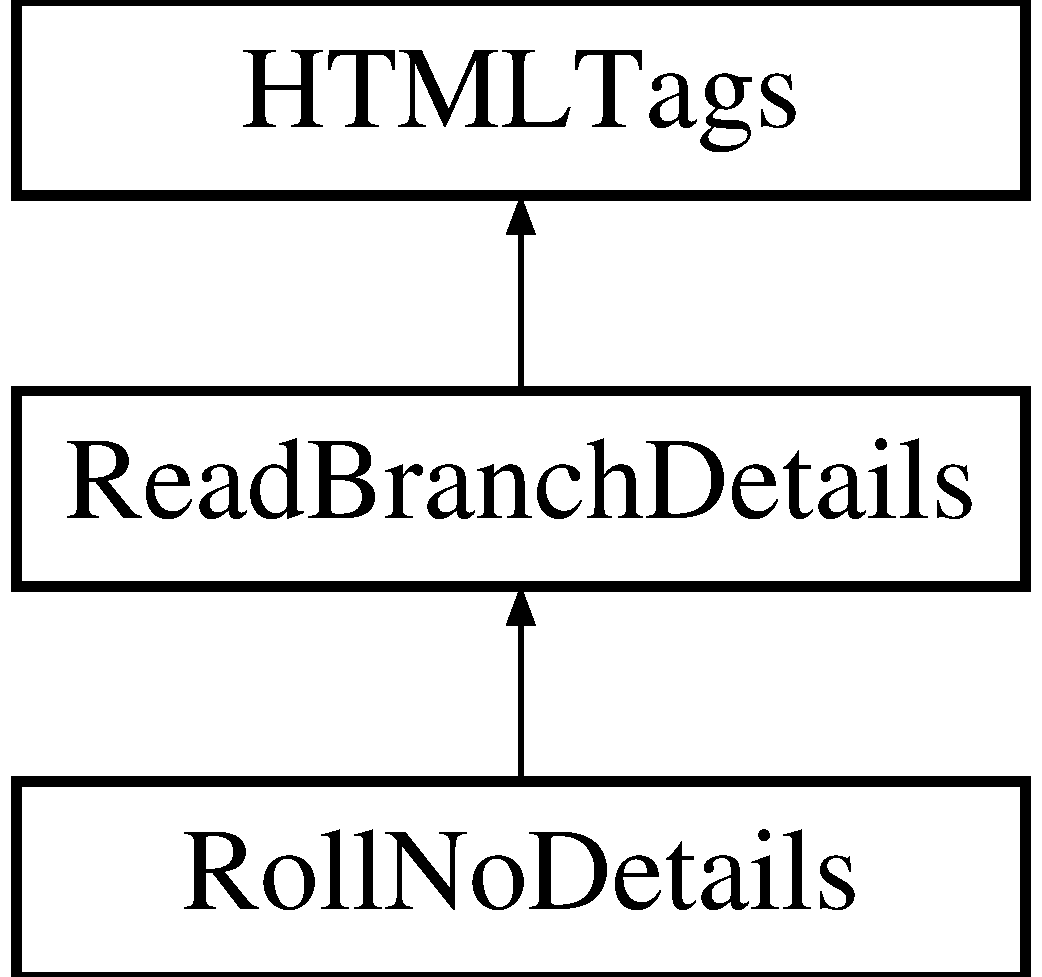
\includegraphics[height=3.000000cm]{classReadBranchDetails}
\end{center}
\end{figure}
\subsection*{Public Member Functions}
\begin{DoxyCompactItemize}
\item 
\hypertarget{classReadBranchDetails_a30c9dd7ace2e554db1f94728ff7d537d}{string {\bfseries read\-Field} (string, int)}\label{classReadBranchDetails_a30c9dd7ace2e554db1f94728ff7d537d}

\item 
\hypertarget{classReadBranchDetails_a1d863278ab0f08e9269237526d9fe9ed}{void {\bfseries read\-Branch\-Details} ()}\label{classReadBranchDetails_a1d863278ab0f08e9269237526d9fe9ed}

\item 
\hypertarget{classReadBranchDetails_a93a178fe62791ae6e9e4c5e814432875}{void {\bfseries write\-Branch\-Details} ()}\label{classReadBranchDetails_a93a178fe62791ae6e9e4c5e814432875}

\item 
\hypertarget{classReadBranchDetails_a074e5d092ba4db817ad012332e525723}{void {\bfseries split\-Sujects} ()}\label{classReadBranchDetails_a074e5d092ba4db817ad012332e525723}

\item 
\hypertarget{classReadBranchDetails_ac82cd5c501b266c24d5d2dbbcc1f2549}{void {\bfseries Main} ()}\label{classReadBranchDetails_ac82cd5c501b266c24d5d2dbbcc1f2549}

\end{DoxyCompactItemize}
\subsection*{Protected Attributes}
\begin{DoxyCompactItemize}
\item 
\hypertarget{classReadBranchDetails_a3454b3b4a6ea8c41727f9720fc9e091a}{int {\bfseries total\-Branches}}\label{classReadBranchDetails_a3454b3b4a6ea8c41727f9720fc9e091a}

\item 
\hypertarget{classReadBranchDetails_a59b8eeaa46e9e26dcde52c952f48f31e}{int {\bfseries total\-Subjects} \mbox{[}M\-I\-N\-S\-\_\-\-S\-I\-Z\-E\mbox{]}}\label{classReadBranchDetails_a59b8eeaa46e9e26dcde52c952f48f31e}

\item 
\hypertarget{classReadBranchDetails_a6e3cae6c059d37b2570729da82c2ea46}{string {\bfseries branch\-Name} \mbox{[}M\-I\-N\-S\-\_\-\-S\-I\-Z\-E\mbox{]}}\label{classReadBranchDetails_a6e3cae6c059d37b2570729da82c2ea46}

\item 
\hypertarget{classReadBranchDetails_aea3079c6dbc33a98f6dd77a625683a48}{string {\bfseries subject\-Name} \mbox{[}M\-I\-N\-S\-\_\-\-S\-I\-Z\-E\mbox{]}\mbox{[}M\-I\-N\-S\-\_\-\-S\-I\-Z\-E\mbox{]}}\label{classReadBranchDetails_aea3079c6dbc33a98f6dd77a625683a48}

\item 
\hypertarget{classReadBranchDetails_a8b56c2864f91301eda7c5a23b2a4ff03}{string {\bfseries subject\-Code} \mbox{[}M\-I\-N\-S\-\_\-\-S\-I\-Z\-E\mbox{]}\mbox{[}M\-I\-N\-S\-\_\-\-S\-I\-Z\-E\mbox{]}}\label{classReadBranchDetails_a8b56c2864f91301eda7c5a23b2a4ff03}

\item 
\hypertarget{classReadBranchDetails_a9b0ae22c37569561b2af60ec48c26694}{string {\bfseries subjectcode} \mbox{[}M\-I\-N\-S\-\_\-\-S\-I\-Z\-E\mbox{]}}\label{classReadBranchDetails_a9b0ae22c37569561b2af60ec48c26694}

\item 
\hypertarget{classReadBranchDetails_a29ea18a15c1978dea055fa3190ce9cba}{string {\bfseries subjectname} \mbox{[}M\-I\-N\-S\-\_\-\-S\-I\-Z\-E\mbox{]}}\label{classReadBranchDetails_a29ea18a15c1978dea055fa3190ce9cba}

\item 
\hypertarget{classReadBranchDetails_a3ca6bc0951aaa5bddcb87d773d23f7eb}{string {\bfseries temp}}\label{classReadBranchDetails_a3ca6bc0951aaa5bddcb87d773d23f7eb}

\item 
\hypertarget{classReadBranchDetails_a7bb99a6ec821f098371df4cb65ab8f65}{Cgicc {\bfseries form\-Data}}\label{classReadBranchDetails_a7bb99a6ec821f098371df4cb65ab8f65}

\item 
\hypertarget{classReadBranchDetails_a6ffffa42ad379f516a3419496469a0d6}{form\-\_\-iterator {\bfseries fi}}\label{classReadBranchDetails_a6ffffa42ad379f516a3419496469a0d6}

\item 
\hypertarget{classReadBranchDetails_afc1d050b96d76aa1e3a8f31a39f7658b}{int {\bfseries total\-Fields}}\label{classReadBranchDetails_afc1d050b96d76aa1e3a8f31a39f7658b}

\end{DoxyCompactItemize}


\subsection{Detailed Description}


Definition at line 3 of file rollnodetails.\-h.



The documentation for this class was generated from the following files\-:\begin{DoxyCompactItemize}
\item 
Baka\-Plan/rollnodetails.\-h\item 
Baka\-Plan/readbranchdetails.\-cc\end{DoxyCompactItemize}

\hypertarget{classReadExamDetails}{\section{Read\-Exam\-Details Class Reference}
\label{classReadExamDetails}\index{Read\-Exam\-Details@{Read\-Exam\-Details}}
}
Inheritance diagram for Read\-Exam\-Details\-:\begin{figure}[H]
\begin{center}
\leavevmode
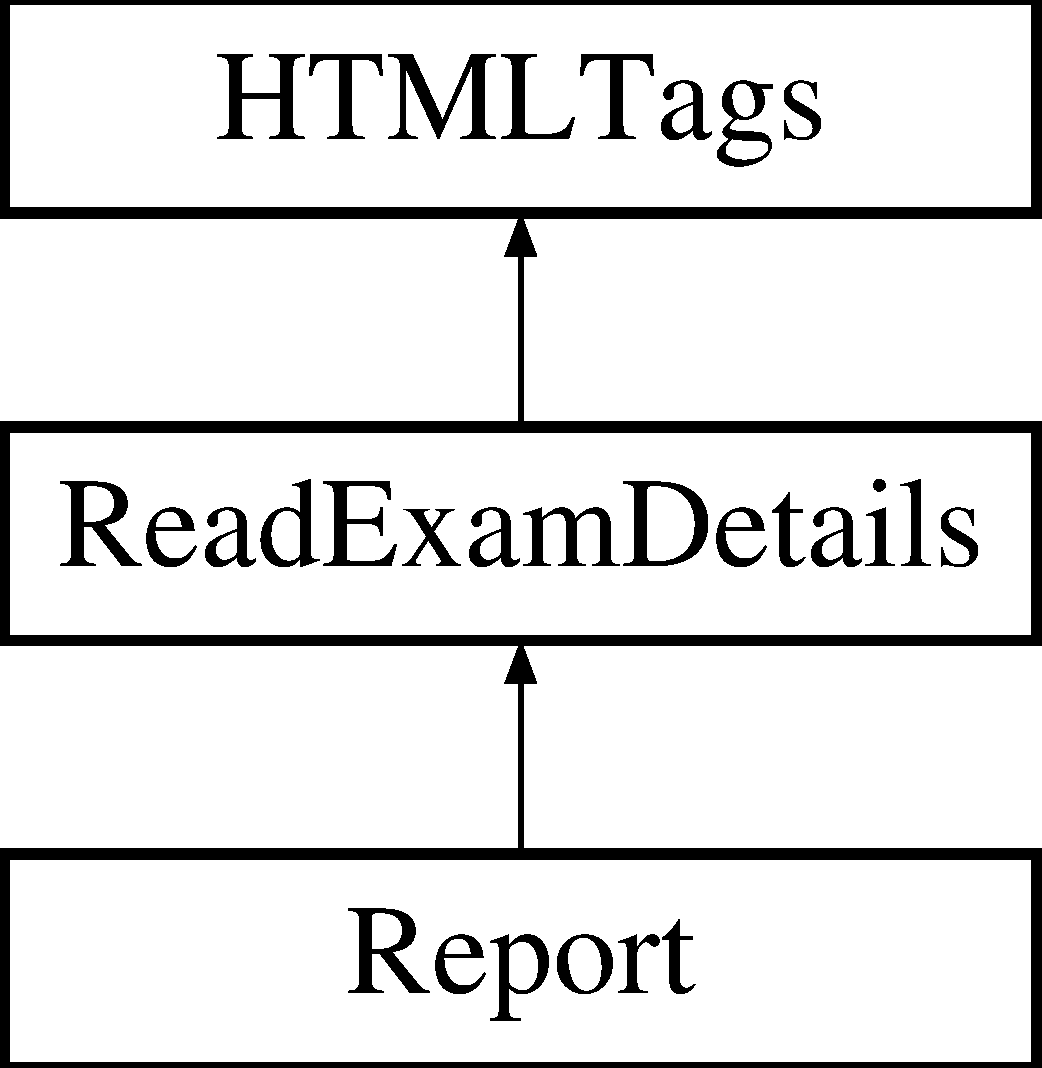
\includegraphics[height=3.000000cm]{classReadExamDetails}
\end{center}
\end{figure}
\subsection*{Public Member Functions}
\begin{DoxyCompactItemize}
\item 
\hypertarget{classReadExamDetails_a419ea4ab2644a1c517f389b726408384}{void {\bfseries read\-Exam\-Details} ()}\label{classReadExamDetails_a419ea4ab2644a1c517f389b726408384}

\item 
\hypertarget{classReadExamDetails_a25941733e41fec97688c730711768a56}{void {\bfseries write\-Exam\-Details} ()}\label{classReadExamDetails_a25941733e41fec97688c730711768a56}

\item 
\hypertarget{classReadExamDetails_a67581721d40087cb5f87000654f02731}{string {\bfseries read\-Field} (string)}\label{classReadExamDetails_a67581721d40087cb5f87000654f02731}

\item 
\hypertarget{classReadExamDetails_a83761c8c6a10b7198054a723b53af9fb}{void {\bfseries Main} ()}\label{classReadExamDetails_a83761c8c6a10b7198054a723b53af9fb}

\end{DoxyCompactItemize}
\subsection*{Protected Attributes}
\begin{DoxyCompactItemize}
\item 
\hypertarget{classReadExamDetails_a815896608a58b449b451305306dd8d38}{string {\bfseries exam\-Name}}\label{classReadExamDetails_a815896608a58b449b451305306dd8d38}

\item 
\hypertarget{classReadExamDetails_a66cd09674039e76f3137d08fea2d9ef2}{string {\bfseries exam\-Date}}\label{classReadExamDetails_a66cd09674039e76f3137d08fea2d9ef2}

\item 
\hypertarget{classReadExamDetails_a86b8b41b014ce26c12113b49137520ef}{string {\bfseries exam\-Time}}\label{classReadExamDetails_a86b8b41b014ce26c12113b49137520ef}

\item 
\hypertarget{classReadExamDetails_a0ef2238b4dd4e930b278658fcf184b73}{string {\bfseries exam\-Venue}}\label{classReadExamDetails_a0ef2238b4dd4e930b278658fcf184b73}

\item 
\hypertarget{classReadExamDetails_a7dff5b6a855ccacaf477b3dd79850c91}{Cgicc {\bfseries form\-Data}}\label{classReadExamDetails_a7dff5b6a855ccacaf477b3dd79850c91}

\item 
\hypertarget{classReadExamDetails_a2d108fa7b89860260891d1fc13329153}{form\-\_\-iterator {\bfseries fi}}\label{classReadExamDetails_a2d108fa7b89860260891d1fc13329153}

\item 
\hypertarget{classReadExamDetails_a77167675e8c30ba10941b7e36866e08e}{string {\bfseries temp}}\label{classReadExamDetails_a77167675e8c30ba10941b7e36866e08e}

\end{DoxyCompactItemize}


The documentation for this class was generated from the following files\-:\begin{DoxyCompactItemize}
\item 
report.\-h\item 
readexamdetails.\-cc\end{DoxyCompactItemize}

\hypertarget{classReadInput}{\section{Read\-Input Class Reference}
\label{classReadInput}\index{Read\-Input@{Read\-Input}}
}


\subsection{Detailed Description}
Include readinput.\-h file 

The documentation for this class was generated from the following file\-:\begin{DoxyCompactItemize}
\item 
frontend/src/backend/\hyperlink{readinput_8cc}{readinput.\-cc}\end{DoxyCompactItemize}

\hypertarget{classReadRollNoDetails}{\section{Read\-Roll\-No\-Details Class Reference}
\label{classReadRollNoDetails}\index{Read\-Roll\-No\-Details@{Read\-Roll\-No\-Details}}
}
Inheritance diagram for Read\-Roll\-No\-Details\-:\begin{figure}[H]
\begin{center}
\leavevmode
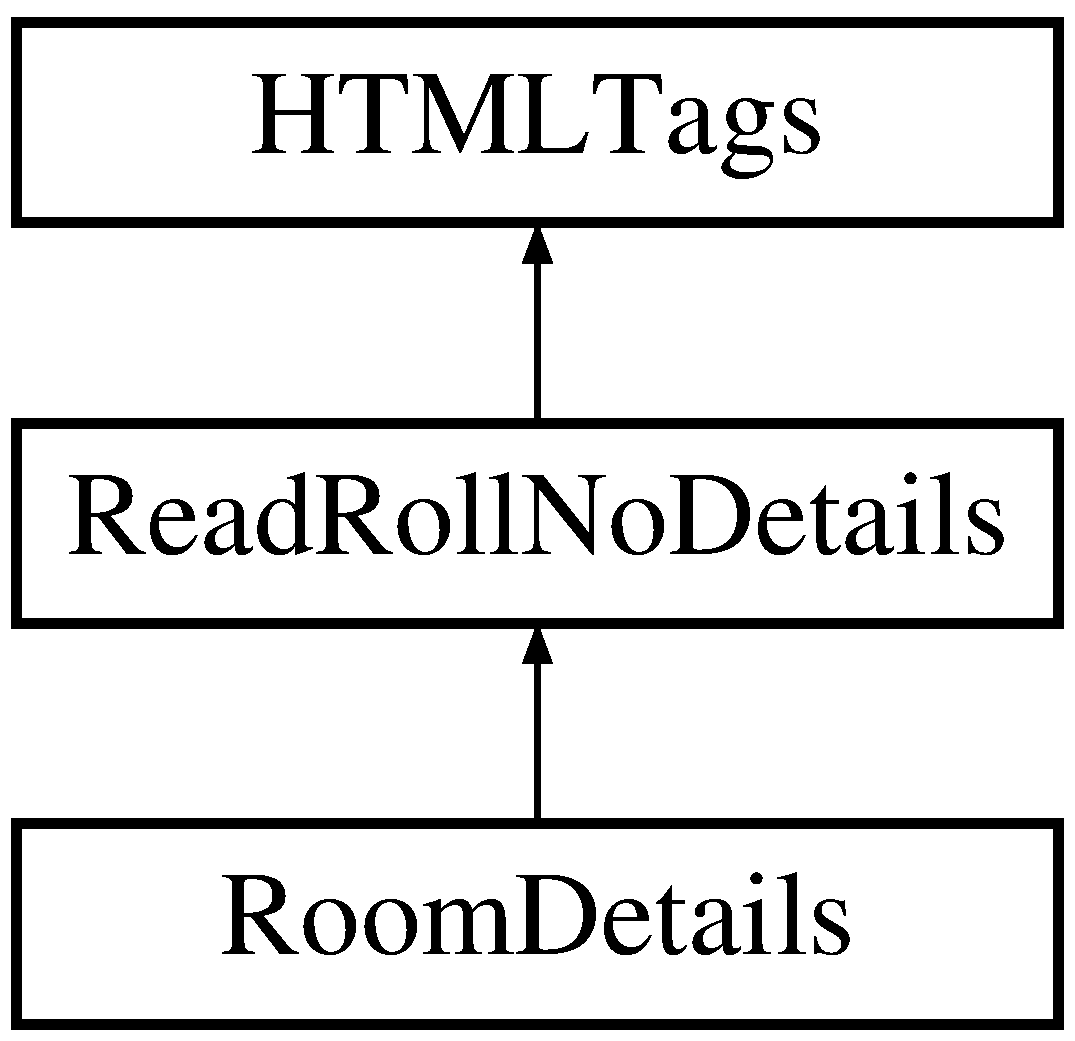
\includegraphics[height=3.000000cm]{classReadRollNoDetails}
\end{center}
\end{figure}
\subsection*{Public Member Functions}
\begin{DoxyCompactItemize}
\item 
\hypertarget{classReadRollNoDetails_a33bc88ab536496022de32f5e30eec0cc}{void {\bfseries read\-Roll\-No\-Details} ()}\label{classReadRollNoDetails_a33bc88ab536496022de32f5e30eec0cc}

\item 
\hypertarget{classReadRollNoDetails_a654f176cecdaed1e661d5ad753ddcb2a}{string {\bfseries read\-Field} (string fieldname, int i)}\label{classReadRollNoDetails_a654f176cecdaed1e661d5ad753ddcb2a}

\item 
\hypertarget{classReadRollNoDetails_a3ebd536e65d2be0909d21420d1cef656}{void {\bfseries write\-Roll\-No\-Details} ()}\label{classReadRollNoDetails_a3ebd536e65d2be0909d21420d1cef656}

\item 
\hypertarget{classReadRollNoDetails_a38a5d6fd6704c950ded2913385a58d0b}{void {\bfseries Main} ()}\label{classReadRollNoDetails_a38a5d6fd6704c950ded2913385a58d0b}

\end{DoxyCompactItemize}
\subsection*{Protected Attributes}
\begin{DoxyCompactItemize}
\item 
\hypertarget{classReadRollNoDetails_a9e3da16b31935dc91fec7c5c9fe5b0b1}{int {\bfseries total\-Fields}}\label{classReadRollNoDetails_a9e3da16b31935dc91fec7c5c9fe5b0b1}

\item 
\hypertarget{classReadRollNoDetails_a3ce491bf8fbdc887b3fc2c1d9bab03f6}{string {\bfseries rno\-Prefix} \mbox{[}M\-I\-N\-S\-\_\-\-S\-I\-Z\-E\mbox{]}}\label{classReadRollNoDetails_a3ce491bf8fbdc887b3fc2c1d9bab03f6}

\item 
\hypertarget{classReadRollNoDetails_a40301d363dead62c878a501f6cc13f3c}{string {\bfseries start\-Roll\-No} \mbox{[}M\-I\-N\-S\-\_\-\-S\-I\-Z\-E\mbox{]}}\label{classReadRollNoDetails_a40301d363dead62c878a501f6cc13f3c}

\item 
\hypertarget{classReadRollNoDetails_a165f0453148ac33fc3d42a0749c1e3d2}{string {\bfseries end\-Roll\-No} \mbox{[}M\-I\-N\-S\-\_\-\-S\-I\-Z\-E\mbox{]}}\label{classReadRollNoDetails_a165f0453148ac33fc3d42a0749c1e3d2}

\item 
\hypertarget{classReadRollNoDetails_add8c46be1edcce9f5d03d0a738d90682}{string {\bfseries not\-Included\-Roll\-No} \mbox{[}M\-I\-N\-S\-\_\-\-S\-I\-Z\-E\mbox{]}}\label{classReadRollNoDetails_add8c46be1edcce9f5d03d0a738d90682}

\item 
\hypertarget{classReadRollNoDetails_ac821611109cf5b331fa827c6c0814176}{Cgicc {\bfseries form\-Data}}\label{classReadRollNoDetails_ac821611109cf5b331fa827c6c0814176}

\item 
\hypertarget{classReadRollNoDetails_a993462dcd9f13d5ab4d0ac41ce58c2c0}{form\-\_\-iterator {\bfseries fi}}\label{classReadRollNoDetails_a993462dcd9f13d5ab4d0ac41ce58c2c0}

\item 
\hypertarget{classReadRollNoDetails_ad362d259f2383fa1c0ee6aef9399b613}{string {\bfseries temp}}\label{classReadRollNoDetails_ad362d259f2383fa1c0ee6aef9399b613}

\end{DoxyCompactItemize}


The documentation for this class was generated from the following files\-:\begin{DoxyCompactItemize}
\item 
roomdetails.\-h\item 
readrollnodetails.\-cc\end{DoxyCompactItemize}

\hypertarget{classReadRoomDetails}{\section{Read\-Room\-Details Class Reference}
\label{classReadRoomDetails}\index{Read\-Room\-Details@{Read\-Room\-Details}}
}
Inheritance diagram for Read\-Room\-Details\-:\begin{figure}[H]
\begin{center}
\leavevmode
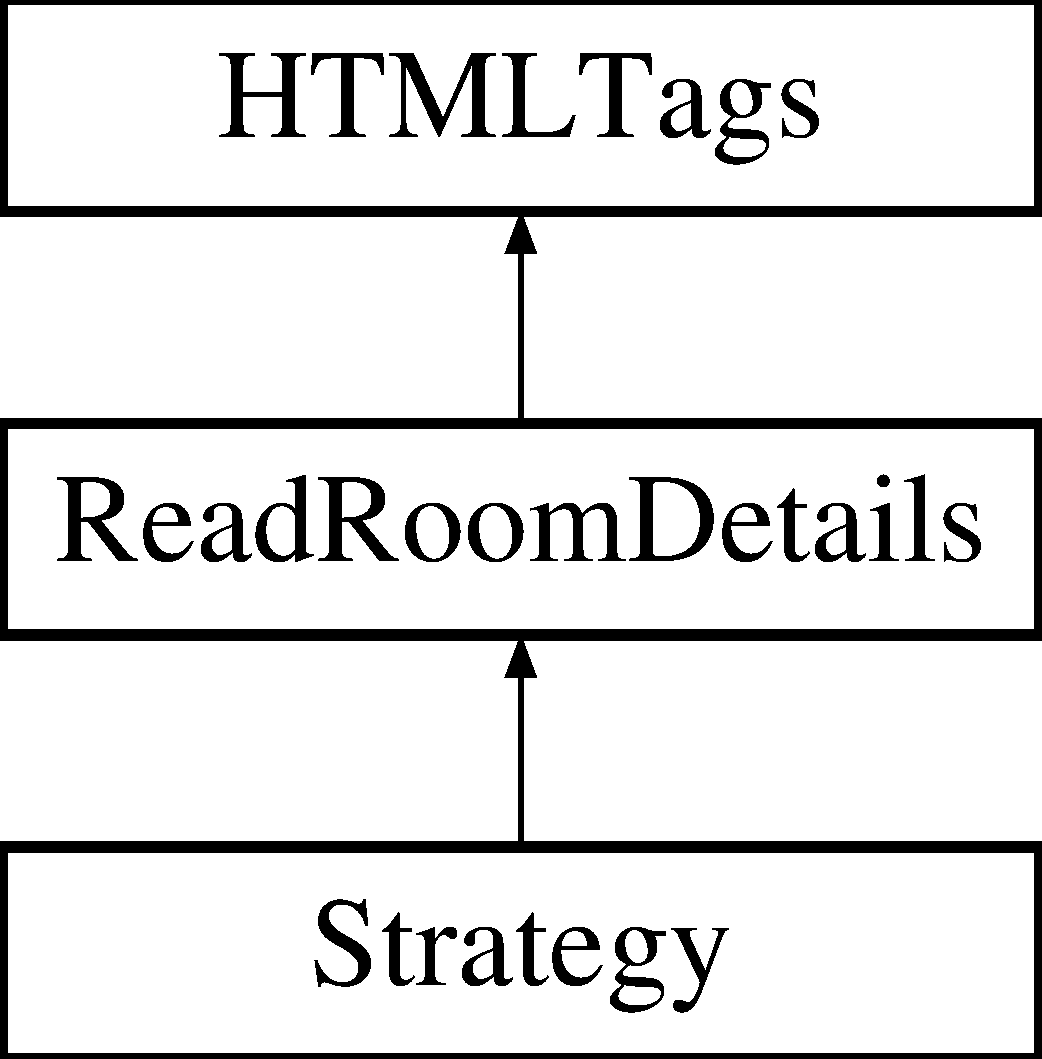
\includegraphics[height=3.000000cm]{classReadRoomDetails}
\end{center}
\end{figure}
\subsection*{Public Member Functions}
\begin{DoxyCompactItemize}
\item 
\hypertarget{classReadRoomDetails_a64f4053481ddccc38b0a3e10d1e126e8}{void {\bfseries read\-Room\-Details} ()}\label{classReadRoomDetails_a64f4053481ddccc38b0a3e10d1e126e8}

\item 
\hypertarget{classReadRoomDetails_ad791618ab41f2eaabb560fdc821d378b}{string {\bfseries read\-Field} (string, int)}\label{classReadRoomDetails_ad791618ab41f2eaabb560fdc821d378b}

\item 
\hypertarget{classReadRoomDetails_ac342a03330fd3a959aabdcebf4dde04c}{string {\bfseries read\-Field} (string, int, int)}\label{classReadRoomDetails_ac342a03330fd3a959aabdcebf4dde04c}

\item 
\hypertarget{classReadRoomDetails_a1a953228597d45f1346ea0b974b3cf1a}{void {\bfseries write\-Room\-Details} ()}\label{classReadRoomDetails_a1a953228597d45f1346ea0b974b3cf1a}

\item 
\hypertarget{classReadRoomDetails_a0492ff264c9960310b181225d008092c}{void {\bfseries Main} ()}\label{classReadRoomDetails_a0492ff264c9960310b181225d008092c}

\end{DoxyCompactItemize}
\subsection*{Protected Attributes}
\begin{DoxyCompactItemize}
\item 
\hypertarget{classReadRoomDetails_aa129e39384751672b59549d8157208a3}{int {\bfseries total\-Centres}}\label{classReadRoomDetails_aa129e39384751672b59549d8157208a3}

\item 
\hypertarget{classReadRoomDetails_ace321366b4a5a91343476cf2c3918eda}{int {\bfseries total\-Rooms} \mbox{[}M\-I\-N\-S\-\_\-\-S\-I\-Z\-E\mbox{]}}\label{classReadRoomDetails_ace321366b4a5a91343476cf2c3918eda}

\item 
\hypertarget{classReadRoomDetails_a7d3fe4925d9d1d61cd1203252fa9520a}{string {\bfseries centre\-No} \mbox{[}M\-I\-N\-S\-\_\-\-S\-I\-Z\-E\mbox{]}}\label{classReadRoomDetails_a7d3fe4925d9d1d61cd1203252fa9520a}

\item 
\hypertarget{classReadRoomDetails_a6b961c05b5c5980de07caec15b25f586}{string {\bfseries room\-No} \mbox{[}M\-I\-N\-S\-\_\-\-S\-I\-Z\-E\mbox{]}\mbox{[}M\-I\-N\-S\-\_\-\-S\-I\-Z\-E\mbox{]}}\label{classReadRoomDetails_a6b961c05b5c5980de07caec15b25f586}

\item 
\hypertarget{classReadRoomDetails_a751d5a539f14f7b1541f24add1a14a8d}{string {\bfseries room\-Rows} \mbox{[}M\-I\-N\-S\-\_\-\-S\-I\-Z\-E\mbox{]}\mbox{[}M\-I\-N\-S\-\_\-\-S\-I\-Z\-E\mbox{]}}\label{classReadRoomDetails_a751d5a539f14f7b1541f24add1a14a8d}

\item 
\hypertarget{classReadRoomDetails_ac9515b760d3bab39cac3673cd276042b}{string {\bfseries room\-Cols} \mbox{[}M\-I\-N\-S\-\_\-\-S\-I\-Z\-E\mbox{]}\mbox{[}M\-I\-N\-S\-\_\-\-S\-I\-Z\-E\mbox{]}}\label{classReadRoomDetails_ac9515b760d3bab39cac3673cd276042b}

\item 
\hypertarget{classReadRoomDetails_a38c9a8165ce1c8078e7843d44a1ba579}{Cgicc {\bfseries form\-Data}}\label{classReadRoomDetails_a38c9a8165ce1c8078e7843d44a1ba579}

\item 
\hypertarget{classReadRoomDetails_a692d9310d1600a6e3bd6cb13247f5ce9}{form\-\_\-iterator {\bfseries fi}}\label{classReadRoomDetails_a692d9310d1600a6e3bd6cb13247f5ce9}

\item 
\hypertarget{classReadRoomDetails_a9d88537ba17a59fb1b1fd54730867969}{string {\bfseries temp}}\label{classReadRoomDetails_a9d88537ba17a59fb1b1fd54730867969}

\item 
\hypertarget{classReadRoomDetails_af3be33bcb331aeca2637e920eced2732}{string {\bfseries strategy\-Name} \mbox{[}M\-I\-N\-S\-\_\-\-S\-I\-Z\-E\mbox{]}}\label{classReadRoomDetails_af3be33bcb331aeca2637e920eced2732}

\end{DoxyCompactItemize}


\subsection{Detailed Description}


Definition at line 3 of file strategy.\-h.



The documentation for this class was generated from the following files\-:\begin{DoxyCompactItemize}
\item 
Baka\-Plan/strategy.\-h\item 
Baka\-Plan/readroomdetails.\-cc\end{DoxyCompactItemize}

\hypertarget{classReport}{\section{Report Class Reference}
\label{classReport}\index{Report@{Report}}
}
Inheritance diagram for Report\-:\begin{figure}[H]
\begin{center}
\leavevmode
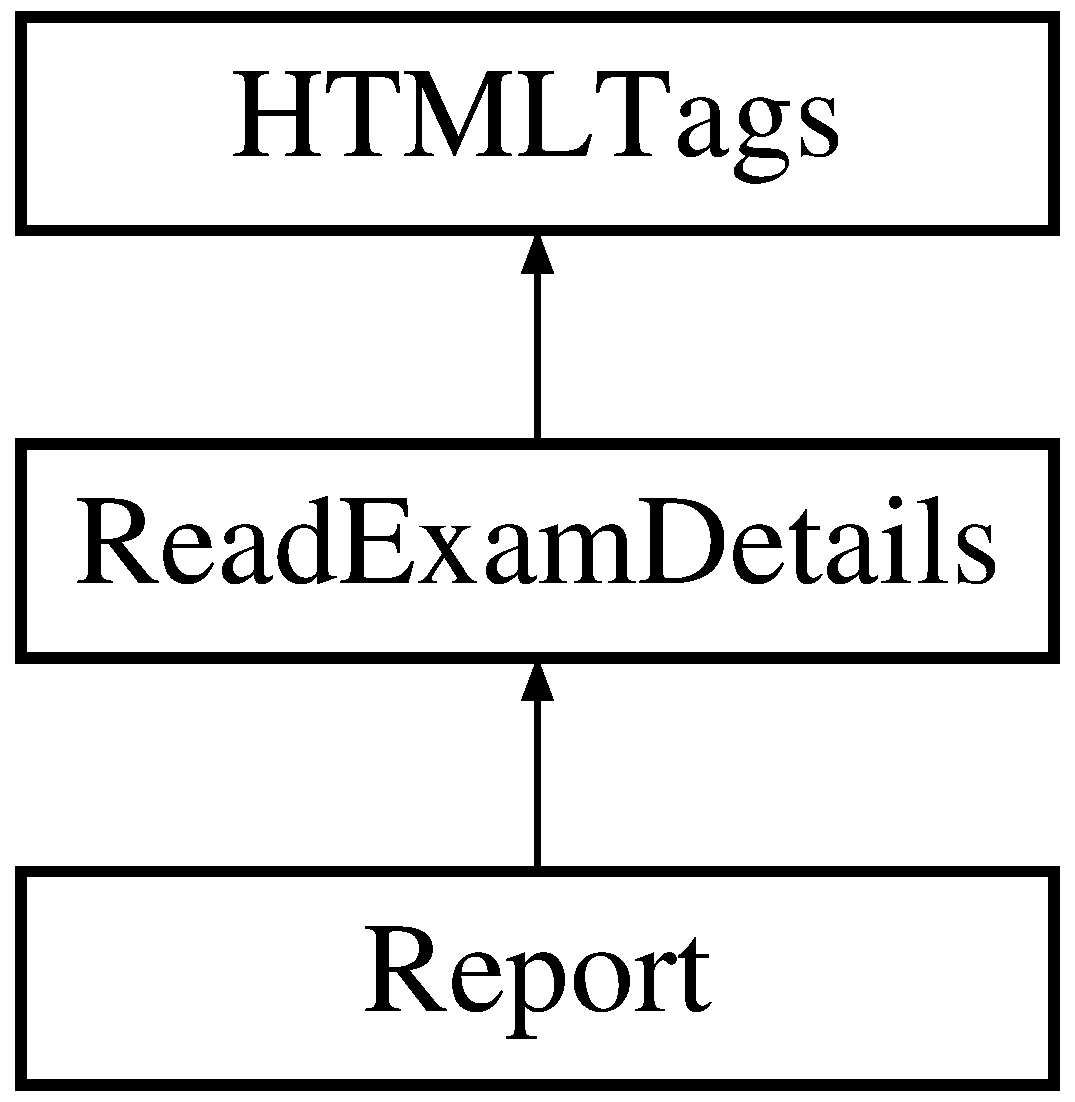
\includegraphics[height=3.000000cm]{classReport}
\end{center}
\end{figure}
\subsection*{Public Member Functions}
\begin{DoxyCompactItemize}
\item 
\hypertarget{classReport_a6b5a749dcbc19cb71503c5a6e2d465d3}{void {\bfseries Head} ()}\label{classReport_a6b5a749dcbc19cb71503c5a6e2d465d3}

\item 
\hypertarget{classReport_a97998b106d6fb7d6ccfea849892d21ee}{void {\bfseries Javascript} ()}\label{classReport_a97998b106d6fb7d6ccfea849892d21ee}

\item 
\hypertarget{classReport_a28dfc98e680194276c2bbb2fa4decf86}{void {\bfseries Body} ()}\label{classReport_a28dfc98e680194276c2bbb2fa4decf86}

\item 
\hypertarget{classReport_abfacfc97c910b8c2bc1a1102cc623d80}{void {\bfseries Body\-Content} ()}\label{classReport_abfacfc97c910b8c2bc1a1102cc623d80}

\item 
\hypertarget{classReport_a35895231f3a27c3247f9498cda2b42fe}{void {\bfseries Main} ()}\label{classReport_a35895231f3a27c3247f9498cda2b42fe}

\end{DoxyCompactItemize}
\subsection*{Additional Inherited Members}


The documentation for this class was generated from the following files\-:\begin{DoxyCompactItemize}
\item 
Baka\-Plan/report.\-h\item 
Baka\-Plan/report.\-cc\end{DoxyCompactItemize}

\hypertarget{classRollNoDetails}{\section{Roll\-No\-Details Class Reference}
\label{classRollNoDetails}\index{Roll\-No\-Details@{Roll\-No\-Details}}
}


{\ttfamily \#include $<$rollnodetails.\-h$>$}

\subsection*{Public Member Functions}
\begin{DoxyCompactItemize}
\item 
\hyperlink{classRollNoDetails_aef927fa87d8ab659f6a241290936980c}{Roll\-No\-Details} ()
\begin{DoxyCompactList}\small\item\em Constructor. \end{DoxyCompactList}\item 
\hyperlink{classRollNoDetails_a218c683c86ee19788b868a08af6e210f}{Read\-Class\-Details} ()
\begin{DoxyCompactList}\small\item\em Reading class details from previous page using cgicc. \end{DoxyCompactList}\item 
\hypertarget{classRollNoDetails_ade931d9c426fbd3fd5d8db72b3a55289}{{\bfseries Write\-Class\-Details} ()}\label{classRollNoDetails_ade931d9c426fbd3fd5d8db72b3a55289}

\end{DoxyCompactItemize}
\subsection*{Protected Attributes}
\begin{DoxyCompactItemize}
\item 
string \hyperlink{classRollNoDetails_a2126e353865b8e215513fe17785ef230}{prefix} \mbox{[}M\-I\-N\-\_\-\-S\-I\-Z\-E\mbox{]}
\begin{DoxyCompactList}\small\item\em for storing values of class details \end{DoxyCompactList}\item 
\hypertarget{classRollNoDetails_a441e0e8f352b04e2eb104d8a69d939c2}{string {\bfseries start\-Roll\-No} \mbox{[}M\-I\-N\-\_\-\-S\-I\-Z\-E\mbox{]}}\label{classRollNoDetails_a441e0e8f352b04e2eb104d8a69d939c2}

\item 
\hypertarget{classRollNoDetails_a8231b6d71b73f825f29a84e290d6736b}{string {\bfseries end\-Roll\-No} \mbox{[}M\-I\-N\-\_\-\-S\-I\-Z\-E\mbox{]}}\label{classRollNoDetails_a8231b6d71b73f825f29a84e290d6736b}

\item 
\hypertarget{classRollNoDetails_a1280f14b2160fb396a675bc4ba5fb85d}{string {\bfseries not\-Included} \mbox{[}M\-I\-N\-\_\-\-S\-I\-Z\-E\mbox{]}}\label{classRollNoDetails_a1280f14b2160fb396a675bc4ba5fb85d}

\item 
\hypertarget{classRollNoDetails_aa2d166949084d8f3ba6d8ab70f49282a}{int {\bfseries total\-Classes}}\label{classRollNoDetails_aa2d166949084d8f3ba6d8ab70f49282a}

\end{DoxyCompactItemize}


\subsection{Detailed Description}


 \subsubsection*{Include required header files}



 Class\-: \hyperlink{classRollNoDetails}{Roll\-No\-Details} \subsection*{Description\-: \hyperlink{classRollNoDetails}{Roll\-No\-Details} class for }

Definition at line 33 of file rollnodetails.\-h.



\subsection{Constructor \& Destructor Documentation}
\hypertarget{classRollNoDetails_aef927fa87d8ab659f6a241290936980c}{\index{Roll\-No\-Details@{Roll\-No\-Details}!Roll\-No\-Details@{Roll\-No\-Details}}
\index{Roll\-No\-Details@{Roll\-No\-Details}!RollNoDetails@{Roll\-No\-Details}}
\subsubsection[{Roll\-No\-Details}]{\setlength{\rightskip}{0pt plus 5cm}Roll\-No\-Details\-::\-Roll\-No\-Details (
\begin{DoxyParamCaption}
{}
\end{DoxyParamCaption}
)}}\label{classRollNoDetails_aef927fa87d8ab659f6a241290936980c}


Constructor. 



 \subsubsection*{Include \hyperlink{rollnodetails_8h_source}{rollnodetails.\-h} for \hyperlink{classRollNoDetails}{Roll\-No\-Details} class declaration}

\subsubsection*{Definition of functions \hyperlink{classRollNoDetails}{Roll\-No\-Details} Class}



 Class\-: \hyperlink{classRollNoDetails}{Roll\-No\-Details} Method\-: \hyperlink{classRollNoDetails}{Roll\-No\-Details} \-:\-: \hyperlink{classRollNoDetails_aef927fa87d8ab659f6a241290936980c}{Roll\-No\-Details()} \subsubsection*{Description\-: Constructor}

Definition at line 37 of file rollnodetails.\-cc.



\subsection{Member Function Documentation}
\hypertarget{classRollNoDetails_a218c683c86ee19788b868a08af6e210f}{\index{Roll\-No\-Details@{Roll\-No\-Details}!Read\-Class\-Details@{Read\-Class\-Details}}
\index{Read\-Class\-Details@{Read\-Class\-Details}!RollNoDetails@{Roll\-No\-Details}}
\subsubsection[{Read\-Class\-Details}]{\setlength{\rightskip}{0pt plus 5cm}void Roll\-No\-Details\-::\-Read\-Class\-Details (
\begin{DoxyParamCaption}
{}
\end{DoxyParamCaption}
)}}\label{classRollNoDetails_a218c683c86ee19788b868a08af6e210f}


Reading class details from previous page using cgicc. 



 Class\-: \hyperlink{classRollNoDetails}{Roll\-No\-Details} Method\-: \hyperlink{classRollNoDetails}{Roll\-No\-Details} \-:\-: \hyperlink{classRollNoDetails_a218c683c86ee19788b868a08af6e210f}{Read\-Class\-Details()} \subsubsection*{Description\-: For reading class details from previous page}

Definition at line 50 of file rollnodetails.\-cc.



\subsection{Member Data Documentation}
\hypertarget{classRollNoDetails_a2126e353865b8e215513fe17785ef230}{\index{Roll\-No\-Details@{Roll\-No\-Details}!prefix@{prefix}}
\index{prefix@{prefix}!RollNoDetails@{Roll\-No\-Details}}
\subsubsection[{prefix}]{\setlength{\rightskip}{0pt plus 5cm}string Roll\-No\-Details\-::prefix\mbox{[}M\-I\-N\-\_\-\-S\-I\-Z\-E\mbox{]}\hspace{0.3cm}{\ttfamily [protected]}}}\label{classRollNoDetails_a2126e353865b8e215513fe17785ef230}


for storing values of class details 



Definition at line 37 of file rollnodetails.\-h.



The documentation for this class was generated from the following files\-:\begin{DoxyCompactItemize}
\item 
src/rollnodetails.\-h\item 
src/rollnodetails.\-cc\end{DoxyCompactItemize}

\hypertarget{classRoomDetails}{\section{Room\-Details Class Reference}
\label{classRoomDetails}\index{Room\-Details@{Room\-Details}}
}
Inheritance diagram for Room\-Details\-:\begin{figure}[H]
\begin{center}
\leavevmode
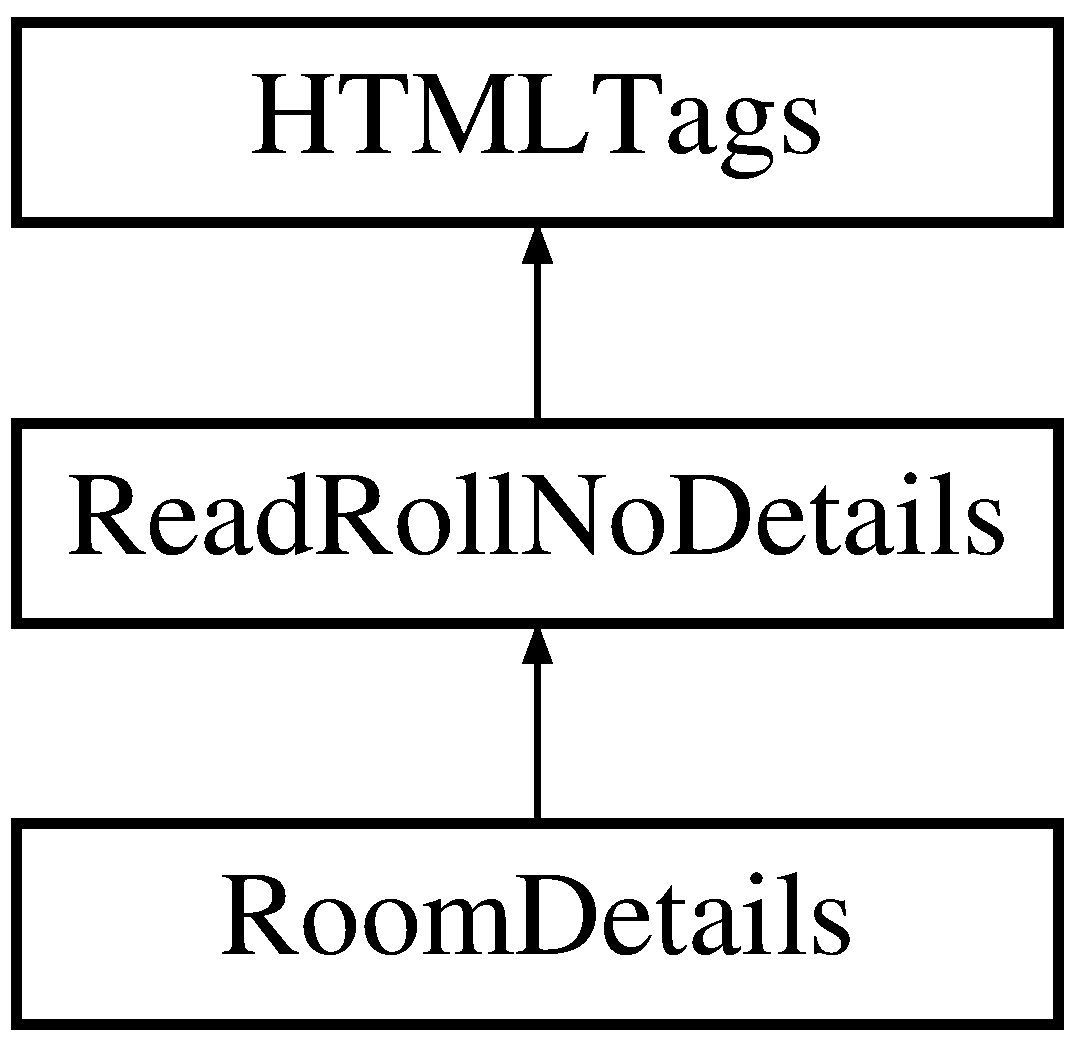
\includegraphics[height=3.000000cm]{classRoomDetails}
\end{center}
\end{figure}
\subsection*{Public Member Functions}
\begin{DoxyCompactItemize}
\item 
\hypertarget{classRoomDetails_a12c87132fd36826fe2af9dbdb0b78e95}{void {\bfseries Head} ()}\label{classRoomDetails_a12c87132fd36826fe2af9dbdb0b78e95}

\item 
\hypertarget{classRoomDetails_aa88baea324517582b52f0e414744ea5d}{void {\bfseries Javascript} ()}\label{classRoomDetails_aa88baea324517582b52f0e414744ea5d}

\item 
\hypertarget{classRoomDetails_ad75c50cee05130e464714649ad640fa5}{void {\bfseries Body} ()}\label{classRoomDetails_ad75c50cee05130e464714649ad640fa5}

\item 
\hypertarget{classRoomDetails_ab440cfe52056a93720c2f6d82622510f}{void {\bfseries Body\-Content} ()}\label{classRoomDetails_ab440cfe52056a93720c2f6d82622510f}

\item 
\hypertarget{classRoomDetails_a5d3f194992c2c13c77d0d07e7d7d5bcd}{void {\bfseries Main} ()}\label{classRoomDetails_a5d3f194992c2c13c77d0d07e7d7d5bcd}

\end{DoxyCompactItemize}
\subsection*{Additional Inherited Members}


The documentation for this class was generated from the following files\-:\begin{DoxyCompactItemize}
\item 
Baka\-Plan/roomdetails.\-h\item 
Baka\-Plan/roomdetails.\-cc\end{DoxyCompactItemize}

\hypertarget{classRoomReport}{\section{Room\-Report Class Reference}
\label{classRoomReport}\index{Room\-Report@{Room\-Report}}
}
Inheritance diagram for Room\-Report\-:\begin{figure}[H]
\begin{center}
\leavevmode
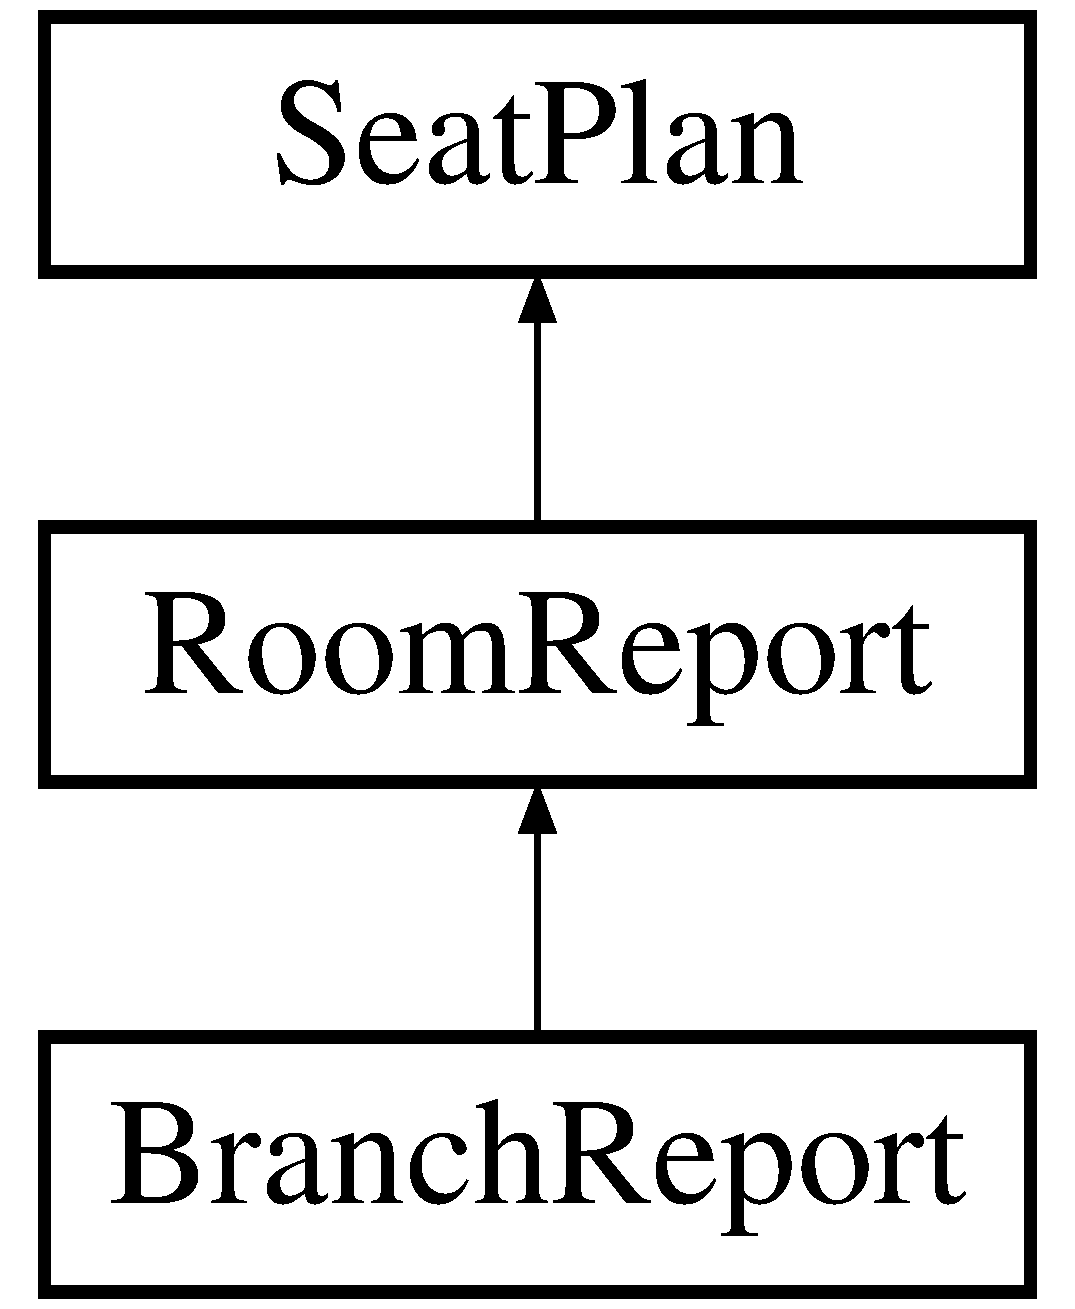
\includegraphics[height=3.000000cm]{classRoomReport}
\end{center}
\end{figure}
\subsection*{Public Member Functions}
\begin{DoxyCompactItemize}
\item 
\hypertarget{classRoomReport_a6befa64df45c74ac5d4810d3b0abdb2c}{void {\bfseries read\-Input\-Roll\-No} (string)}\label{classRoomReport_a6befa64df45c74ac5d4810d3b0abdb2c}

\item 
\hypertarget{classRoomReport_a488ef42cd98cf26383c5753af972dfde}{void {\bfseries read\-Seat\-Plan} (string)}\label{classRoomReport_a488ef42cd98cf26383c5753af972dfde}

\item 
\hypertarget{classRoomReport_a74d8d4a54ab1a80d84c059827ec3c4f6}{void {\bfseries read\-Exam\-Details} (string)}\label{classRoomReport_a74d8d4a54ab1a80d84c059827ec3c4f6}

\item 
\hypertarget{classRoomReport_a3704858e3ace6b7ef0104bdbecf745db}{void {\bfseries write\-Seat\-Plan} (string)}\label{classRoomReport_a3704858e3ace6b7ef0104bdbecf745db}

\item 
\hypertarget{classRoomReport_aa6eff185efa1c6205ec1446ed66d9766}{void {\bfseries Main} ()}\label{classRoomReport_aa6eff185efa1c6205ec1446ed66d9766}

\end{DoxyCompactItemize}
\subsection*{Protected Attributes}
\begin{DoxyCompactItemize}
\item 
\hypertarget{classRoomReport_af342c8a98e579b420ebde3783ad5f3df}{string {\bfseries rollno} \mbox{[}M\-I\-N\-\_\-\-S\-I\-Z\-E\mbox{]}\mbox{[}M\-I\-N\-\_\-\-S\-I\-Z\-E\mbox{]}\mbox{[}M\-A\-X\-\_\-\-S\-I\-Z\-E\mbox{]}}\label{classRoomReport_af342c8a98e579b420ebde3783ad5f3df}

\item 
\hypertarget{classRoomReport_a2582b819b47038641678e4645f25de34}{string {\bfseries branch\-\_\-name} \mbox{[}M\-I\-N\-\_\-\-S\-I\-Z\-E\mbox{]}}\label{classRoomReport_a2582b819b47038641678e4645f25de34}

\item 
\hypertarget{classRoomReport_a530a885bacdce429ae607b741216d4b5}{string {\bfseries subject\-\_\-name} \mbox{[}M\-I\-N\-\_\-\-S\-I\-Z\-E\mbox{]}\mbox{[}M\-I\-N\-\_\-\-S\-I\-Z\-E\mbox{]}}\label{classRoomReport_a530a885bacdce429ae607b741216d4b5}

\item 
\hypertarget{classRoomReport_a62207caf3dd352107bd2566138a98ae4}{string {\bfseries subject\-\_\-code} \mbox{[}M\-I\-N\-\_\-\-S\-I\-Z\-E\mbox{]}\mbox{[}M\-I\-N\-\_\-\-S\-I\-Z\-E\mbox{]}}\label{classRoomReport_a62207caf3dd352107bd2566138a98ae4}

\item 
\hypertarget{classRoomReport_a099a235828672ee6c31dd163d51e648c}{int {\bfseries total\-\_\-rollno} \mbox{[}M\-I\-N\-\_\-\-S\-I\-Z\-E\mbox{]}\mbox{[}M\-I\-N\-\_\-\-S\-I\-Z\-E\mbox{]}}\label{classRoomReport_a099a235828672ee6c31dd163d51e648c}

\item 
\hypertarget{classRoomReport_a4ce1c0593c6d5053575fcf7975ed1577}{int {\bfseries total\-\_\-branches}}\label{classRoomReport_a4ce1c0593c6d5053575fcf7975ed1577}

\item 
\hypertarget{classRoomReport_ad526976fbeecd9b4ad1888e1b90eb9ee}{int {\bfseries total\-\_\-subject} \mbox{[}M\-I\-N\-\_\-\-S\-I\-Z\-E\mbox{]}}\label{classRoomReport_ad526976fbeecd9b4ad1888e1b90eb9ee}

\end{DoxyCompactItemize}


The documentation for this class was generated from the following files\-:\begin{DoxyCompactItemize}
\item 
Baka\-Plan/\-Seat\-Plan/report.\-h\item 
Baka\-Plan/\-Seat\-Plan/room-\/report.\-cc\end{DoxyCompactItemize}

\hypertarget{classSeatPlan}{\section{Seat\-Plan Class Reference}
\label{classSeatPlan}\index{Seat\-Plan@{Seat\-Plan}}
}


\hyperlink{classSeatPlan}{Seat\-Plan} C\-Lass for generating seating plan.  




{\ttfamily \#include $<$report.\-h$>$}

Inheritance diagram for Seat\-Plan\-:\begin{figure}[H]
\begin{center}
\leavevmode
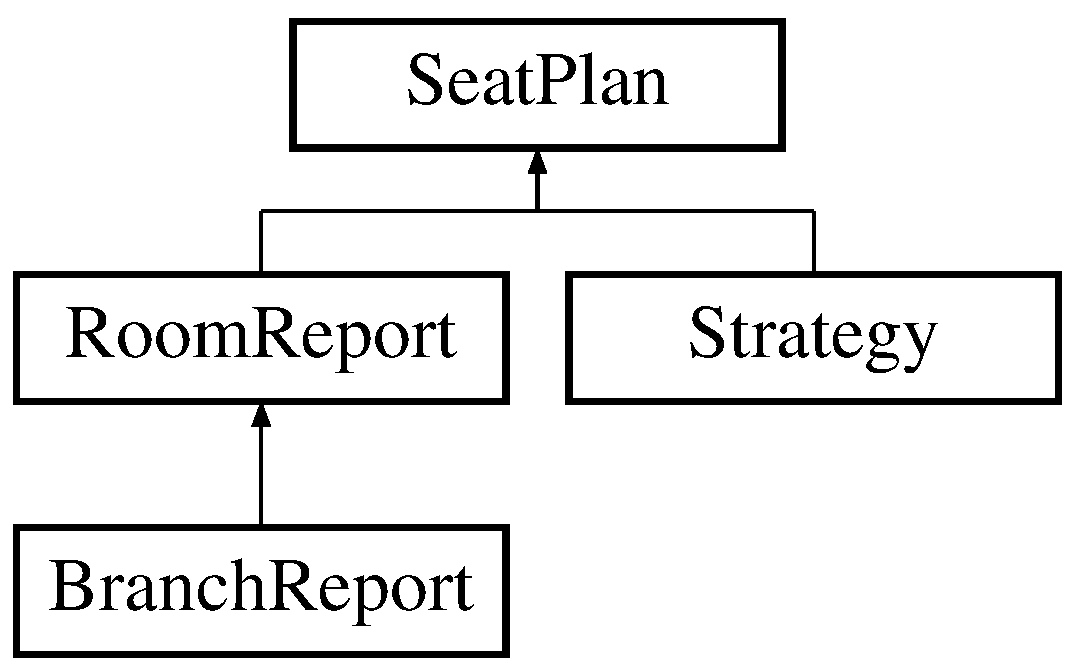
\includegraphics[height=3.000000cm]{classSeatPlan}
\end{center}
\end{figure}
\subsection*{Public Member Functions}
\begin{DoxyCompactItemize}
\item 
\hyperlink{classSeatPlan_a974a336df39c9fefc2b239a382a4749c}{Room\-Report} ()
\item 
void \hyperlink{classSeatPlan_ae93cefd4fd0401c5d54b8e97b23541ae}{Read\-Exam\-Detail} (string \hyperlink{classReadInput_a3ad470a25b3e0a29466bf4ff1f7d8e81}{project\-I\-D})
\item 
void \hyperlink{classSeatPlan_a618d148beefee9d4db3d038328c9b2c8}{Read\-Seat\-Plan} (string \hyperlink{classReadInput_a3ad470a25b3e0a29466bf4ff1f7d8e81}{project\-I\-D})
\item 
void \hyperlink{classSeatPlan_af572f79142f4dad362f54892c6747214}{Write\-H\-T\-M\-L\-File} (string \hyperlink{classReadInput_a3ad470a25b3e0a29466bf4ff1f7d8e81}{project\-I\-D})
\item 
\hyperlink{classSeatPlan_a446949506a25bcda5eb972c8a4b1384d}{$\sim$\-Room\-Report} ()
\item 
\hyperlink{classSeatPlan_ab1906186f96847704ed71f1a6c738327}{Seat\-Plan} ()
\begin{DoxyCompactList}\small\item\em Constructor. \end{DoxyCompactList}\item 
\hypertarget{classSeatPlan_afa418b9edadff831c73ea6005666becf}{void {\bfseries Set\-Roll\-No} (int strategy, int i)}\label{classSeatPlan_afa418b9edadff831c73ea6005666becf}

\item 
\hypertarget{classSeatPlan_a3dfc44c97eab7f3d33f2023ae0faaa13}{string {\bfseries Roll\-No} (int s)}\label{classSeatPlan_a3dfc44c97eab7f3d33f2023ae0faaa13}

\item 
\hypertarget{classSeatPlan_a1df3b03c983936c07225ed1a79959f1b}{void {\bfseries Seating\-Plan} (int strategy, int i)}\label{classSeatPlan_a1df3b03c983936c07225ed1a79959f1b}

\item 
\hypertarget{classSeatPlan_ade684c0f63b648d4d62df8e7ed800682}{void {\bfseries Create\-File} (string \hyperlink{classReadInput_a3ad470a25b3e0a29466bf4ff1f7d8e81}{project\-I\-D})}\label{classSeatPlan_ade684c0f63b648d4d62df8e7ed800682}

\item 
\hypertarget{classSeatPlan_a3f29cad9d9be46f7bc3055de2ab887fc}{void {\bfseries Write\-Seat\-Plan} (string \hyperlink{classReadInput_a3ad470a25b3e0a29466bf4ff1f7d8e81}{project\-I\-D}, int i)}\label{classSeatPlan_a3f29cad9d9be46f7bc3055de2ab887fc}

\item 
void \hyperlink{classSeatPlan_a67c10e2277f1f2823581cddf4df373c5}{Write\-H\-T\-M\-L\-File} (string \hyperlink{classReadInput_a3ad470a25b3e0a29466bf4ff1f7d8e81}{project\-I\-D}, int i)
\begin{DoxyCompactList}\small\item\em Creating H\-T\-M\-L file. \end{DoxyCompactList}\item 
\hypertarget{classSeatPlan_abce0c5b5545f1bb1ebcf2e578b6ab282}{void {\bfseries Write\-P\-D\-F\-File} (string \hyperlink{classReadInput_a3ad470a25b3e0a29466bf4ff1f7d8e81}{project\-I\-D}, int i)}\label{classSeatPlan_abce0c5b5545f1bb1ebcf2e578b6ab282}

\item 
\hypertarget{classSeatPlan_a3257eb25ac9c82d2757d2a7144614762}{void {\bfseries Add\-Roll\-No\-Info} (string \hyperlink{classReadInput_a3ad470a25b3e0a29466bf4ff1f7d8e81}{project\-I\-D}, int i)}\label{classSeatPlan_a3257eb25ac9c82d2757d2a7144614762}

\item 
\hyperlink{classSeatPlan_a373a1d60b6617a2e424f7d2f8866ec2e}{$\sim$\-Seat\-Plan} ()
\begin{DoxyCompactList}\small\item\em D\-Estructor. \end{DoxyCompactList}\end{DoxyCompactItemize}
\subsection*{Protected Attributes}
\begin{DoxyCompactItemize}
\item 
\hypertarget{classSeatPlan_a6915f74be45af73cda8c9a51b6cb99c9}{int {\bfseries total\-Seats}}\label{classSeatPlan_a6915f74be45af73cda8c9a51b6cb99c9}

\item 
\hypertarget{classSeatPlan_a3568dfc375740fd6b4075d7dc419a2e5}{int {\bfseries total\-Students}}\label{classSeatPlan_a3568dfc375740fd6b4075d7dc419a2e5}

\item 
\hypertarget{classSeatPlan_a18b1d6497343d6a9e751159dcdd8a179}{int {\bfseries total\-Group\-Seats}}\label{classSeatPlan_a18b1d6497343d6a9e751159dcdd8a179}

\item 
\hypertarget{classSeatPlan_acf6fa47342ec7f5675064c5601800f5c}{int {\bfseries day}}\label{classSeatPlan_acf6fa47342ec7f5675064c5601800f5c}

\item 
\hypertarget{classSeatPlan_a19a423aff33092a242f5dff5694efa37}{I\-N\-T\-\_\-\-V\-E\-C {\bfseries i\-Temp}}\label{classSeatPlan_a19a423aff33092a242f5dff5694efa37}

\item 
\hypertarget{classSeatPlan_af3fbce455c6744dee3fedb97442cd2c3}{I\-N\-T\-\_\-\-V\-E\-C {\bfseries index\-Value}}\label{classSeatPlan_af3fbce455c6744dee3fedb97442cd2c3}

\item 
\hypertarget{classSeatPlan_a6cb00329d2f0760f679d7e00958da879}{I\-N\-T\-\_\-\-V\-E\-C {\bfseries group\-Student\-Size}}\label{classSeatPlan_a6cb00329d2f0760f679d7e00958da879}

\item 
\hypertarget{classSeatPlan_a73de1d93e86c3a23406e0903c546ea2c}{I\-N\-T\-\_\-\-V\-E\-C {\bfseries seat\-Size}}\label{classSeatPlan_a73de1d93e86c3a23406e0903c546ea2c}

\item 
\hypertarget{classSeatPlan_a45d2c9c1d580d442bc15dcb50265d627}{I\-N\-T\-\_\-\-V\-E\-C {\bfseries size}}\label{classSeatPlan_a45d2c9c1d580d442bc15dcb50265d627}

\item 
\hypertarget{classSeatPlan_a52bafc6123bd54a8f95253c4693b2975}{I\-N\-T\-\_\-3\-D\-V\-E\-C {\bfseries room\-Size}}\label{classSeatPlan_a52bafc6123bd54a8f95253c4693b2975}

\item 
\hypertarget{classSeatPlan_ace374a7f84b7f9fb43fc56979a3793fb}{S\-T\-R\-I\-N\-G\-\_\-\-V\-E\-C {\bfseries sub\-Sub\-Code}}\label{classSeatPlan_ace374a7f84b7f9fb43fc56979a3793fb}

\item 
\hypertarget{classSeatPlan_adf8ed7579be4a43e20cbf4b40bb7b25e}{S\-T\-R\-I\-N\-G\-\_\-2\-D\-V\-E\-C {\bfseries seat\-Roll\-No}}\label{classSeatPlan_adf8ed7579be4a43e20cbf4b40bb7b25e}

\item 
\hypertarget{classSeatPlan_a38f161cde37bcfae5877a17f785cbb21}{S\-T\-R\-I\-N\-G\-\_\-2\-D\-V\-E\-C {\bfseries sub\-Roll\-No}}\label{classSeatPlan_a38f161cde37bcfae5877a17f785cbb21}

\item 
\hypertarget{classSeatPlan_a99f24fdf486af2b45bf142558011573d}{S\-T\-R\-I\-N\-G\-\_\-4\-D\-V\-E\-C {\bfseries seat}}\label{classSeatPlan_a99f24fdf486af2b45bf142558011573d}

\item 
\hypertarget{classSeatPlan_ac623e253b6005a0907c2dab61705f2ab}{int {\bfseries text\-Width}}\label{classSeatPlan_ac623e253b6005a0907c2dab61705f2ab}

\item 
\hypertarget{classSeatPlan_a2e67c39e7c6fff250ce3dc727f0680fd}{int {\bfseries text\-Width1}}\label{classSeatPlan_a2e67c39e7c6fff250ce3dc727f0680fd}

\item 
\hypertarget{classSeatPlan_aff452e60a99eb2582210d3ea7f454a32}{int {\bfseries rect\-Width}}\label{classSeatPlan_aff452e60a99eb2582210d3ea7f454a32}

\item 
\hypertarget{classSeatPlan_a878a765b96afb02615e7eb29bac8678d}{int {\bfseries x}}\label{classSeatPlan_a878a765b96afb02615e7eb29bac8678d}

\item 
\hypertarget{classSeatPlan_ab3a440c8ee63a36610340b1352d69f34}{int {\bfseries y}}\label{classSeatPlan_ab3a440c8ee63a36610340b1352d69f34}

\item 
\hypertarget{classSeatPlan_af13573b0c9227b8bba267fc9f3476f43}{int {\bfseries width}}\label{classSeatPlan_af13573b0c9227b8bba267fc9f3476f43}

\item 
\hypertarget{classSeatPlan_ad7a71523cc34692963985241fe942359}{int {\bfseries height}}\label{classSeatPlan_ad7a71523cc34692963985241fe942359}

\item 
\hypertarget{classSeatPlan_a55052a9b7a637609f439a003b0957552}{int {\bfseries centre}}\label{classSeatPlan_a55052a9b7a637609f439a003b0957552}

\item 
\hypertarget{classSeatPlan_ab01207ceddc85e4535874e2db71e36e3}{int {\bfseries room}}\label{classSeatPlan_ab01207ceddc85e4535874e2db71e36e3}

\item 
\hypertarget{classSeatPlan_a0b1f1e5086e938c3f484bbec62ff0dff}{int {\bfseries room1}}\label{classSeatPlan_a0b1f1e5086e938c3f484bbec62ff0dff}

\item 
\hypertarget{classSeatPlan_afcff743dbcb0e5c364cac4570730ad25}{int {\bfseries row}}\label{classSeatPlan_afcff743dbcb0e5c364cac4570730ad25}

\item 
\hypertarget{classSeatPlan_a959c1e5ee849ea93b5f46a98d4f45060}{int {\bfseries col}}\label{classSeatPlan_a959c1e5ee849ea93b5f46a98d4f45060}

\item 
\hypertarget{classSeatPlan_a31abf30876cae554e4a11f3b4892a93c}{int {\bfseries s}}\label{classSeatPlan_a31abf30876cae554e4a11f3b4892a93c}

\item 
\hypertarget{classSeatPlan_a03348c2da937f350737d7039dbd80cc8}{int {\bfseries start}}\label{classSeatPlan_a03348c2da937f350737d7039dbd80cc8}

\item 
\hypertarget{classSeatPlan_ade0c58a66a04c9f90803dee62954e15f}{int {\bfseries end}}\label{classSeatPlan_ade0c58a66a04c9f90803dee62954e15f}

\item 
\hypertarget{classSeatPlan_a2c85aa97b3681f2ba5e27af197836b26}{int {\bfseries index}}\label{classSeatPlan_a2c85aa97b3681f2ba5e27af197836b26}

\end{DoxyCompactItemize}


\subsection{Detailed Description}
\hyperlink{classSeatPlan}{Seat\-Plan} C\-Lass for generating seating plan. 

Include local header file

include \hyperlink{readinput_8h}{readinput.\-h}

include \hyperlink{seatplan_8h}{seatplan.\-h} file 

Definition at line 25 of file report.\-h.



\subsection{Constructor \& Destructor Documentation}
\hypertarget{classSeatPlan_a446949506a25bcda5eb972c8a4b1384d}{\index{Seat\-Plan@{Seat\-Plan}!$\sim$\-Room\-Report@{$\sim$\-Room\-Report}}
\index{$\sim$\-Room\-Report@{$\sim$\-Room\-Report}!SeatPlan@{Seat\-Plan}}
\subsubsection[{$\sim$\-Room\-Report}]{\setlength{\rightskip}{0pt plus 5cm}Seat\-Plan\-::$\sim$\-Room\-Report (
\begin{DoxyParamCaption}
{}
\end{DoxyParamCaption}
)}}\label{classSeatPlan_a446949506a25bcda5eb972c8a4b1384d}
Destructor \hypertarget{classSeatPlan_ab1906186f96847704ed71f1a6c738327}{\index{Seat\-Plan@{Seat\-Plan}!Seat\-Plan@{Seat\-Plan}}
\index{Seat\-Plan@{Seat\-Plan}!SeatPlan@{Seat\-Plan}}
\subsubsection[{Seat\-Plan}]{\setlength{\rightskip}{0pt plus 5cm}Seat\-Plan\-::\-Seat\-Plan (
\begin{DoxyParamCaption}
{}
\end{DoxyParamCaption}
)}}\label{classSeatPlan_ab1906186f96847704ed71f1a6c738327}


Constructor. 

Constructor 

Definition at line 28 of file seatplan.\-cc.

\hypertarget{classSeatPlan_a373a1d60b6617a2e424f7d2f8866ec2e}{\index{Seat\-Plan@{Seat\-Plan}!$\sim$\-Seat\-Plan@{$\sim$\-Seat\-Plan}}
\index{$\sim$\-Seat\-Plan@{$\sim$\-Seat\-Plan}!SeatPlan@{Seat\-Plan}}
\subsubsection[{$\sim$\-Seat\-Plan}]{\setlength{\rightskip}{0pt plus 5cm}Seat\-Plan\-::$\sim$\-Seat\-Plan (
\begin{DoxyParamCaption}
{}
\end{DoxyParamCaption}
)}}\label{classSeatPlan_a373a1d60b6617a2e424f7d2f8866ec2e}


D\-Estructor. 

Destructor 

Definition at line 593 of file seatplan.\-cc.



\subsection{Member Function Documentation}
\hypertarget{classSeatPlan_ae93cefd4fd0401c5d54b8e97b23541ae}{\index{Seat\-Plan@{Seat\-Plan}!Read\-Exam\-Detail@{Read\-Exam\-Detail}}
\index{Read\-Exam\-Detail@{Read\-Exam\-Detail}!SeatPlan@{Seat\-Plan}}
\subsubsection[{Read\-Exam\-Detail}]{\setlength{\rightskip}{0pt plus 5cm}void Seat\-Plan\-::\-Read\-Exam\-Detail (
\begin{DoxyParamCaption}
\item[{string}]{project\-I\-D}
\end{DoxyParamCaption}
)}}\label{classSeatPlan_ae93cefd4fd0401c5d54b8e97b23541ae}
Read Exam Detail \hypertarget{classSeatPlan_a618d148beefee9d4db3d038328c9b2c8}{\index{Seat\-Plan@{Seat\-Plan}!Read\-Seat\-Plan@{Read\-Seat\-Plan}}
\index{Read\-Seat\-Plan@{Read\-Seat\-Plan}!SeatPlan@{Seat\-Plan}}
\subsubsection[{Read\-Seat\-Plan}]{\setlength{\rightskip}{0pt plus 5cm}void Seat\-Plan\-::\-Read\-Seat\-Plan (
\begin{DoxyParamCaption}
\item[{string}]{project\-I\-D}
\end{DoxyParamCaption}
)}}\label{classSeatPlan_a618d148beefee9d4db3d038328c9b2c8}
Read Seat Plan \hypertarget{classSeatPlan_a974a336df39c9fefc2b239a382a4749c}{\index{Seat\-Plan@{Seat\-Plan}!Room\-Report@{Room\-Report}}
\index{Room\-Report@{Room\-Report}!SeatPlan@{Seat\-Plan}}
\subsubsection[{Room\-Report}]{\setlength{\rightskip}{0pt plus 5cm}Seat\-Plan\-::\-Room\-Report (
\begin{DoxyParamCaption}
{}
\end{DoxyParamCaption}
)}}\label{classSeatPlan_a974a336df39c9fefc2b239a382a4749c}
Constructor \hypertarget{classSeatPlan_af572f79142f4dad362f54892c6747214}{\index{Seat\-Plan@{Seat\-Plan}!Write\-H\-T\-M\-L\-File@{Write\-H\-T\-M\-L\-File}}
\index{Write\-H\-T\-M\-L\-File@{Write\-H\-T\-M\-L\-File}!SeatPlan@{Seat\-Plan}}
\subsubsection[{Write\-H\-T\-M\-L\-File}]{\setlength{\rightskip}{0pt plus 5cm}void Seat\-Plan\-::\-Write\-H\-T\-M\-L\-File (
\begin{DoxyParamCaption}
\item[{string}]{project\-I\-D}
\end{DoxyParamCaption}
)}}\label{classSeatPlan_af572f79142f4dad362f54892c6747214}
Write\-H\-T\-M\-L\-File \hypertarget{classSeatPlan_a67c10e2277f1f2823581cddf4df373c5}{\index{Seat\-Plan@{Seat\-Plan}!Write\-H\-T\-M\-L\-File@{Write\-H\-T\-M\-L\-File}}
\index{Write\-H\-T\-M\-L\-File@{Write\-H\-T\-M\-L\-File}!SeatPlan@{Seat\-Plan}}
\subsubsection[{Write\-H\-T\-M\-L\-File}]{\setlength{\rightskip}{0pt plus 5cm}void Seat\-Plan\-::\-Write\-H\-T\-M\-L\-File (
\begin{DoxyParamCaption}
\item[{string}]{project\-I\-D, }
\item[{int}]{i}
\end{DoxyParamCaption}
)}}\label{classSeatPlan_a67c10e2277f1f2823581cddf4df373c5}


Creating H\-T\-M\-L file. 


\begin{DoxyParams}{Parameters}
{\em project\-I\-D} & Project Id of seating plan project \\
\hline
{\em i} & For creating file accord to datesheet \\
\hline
\end{DoxyParams}


Definition at line 311 of file seatplan.\-cc.



The documentation for this class was generated from the following files\-:\begin{DoxyCompactItemize}
\item 
src/cpp/backend/header/\hyperlink{report_8h}{report.\-h}\item 
src/cpp/backend/header/\hyperlink{seatplan_8h}{seatplan.\-h}\item 
src/cpp/backend/\hyperlink{seatplan_8cc}{seatplan.\-cc}\end{DoxyCompactItemize}

\hypertarget{classStrategy}{\section{Strategy Class Reference}
\label{classStrategy}\index{Strategy@{Strategy}}
}


\subsection{Detailed Description}
include strategy.\-h 

The documentation for this class was generated from the following file\-:\begin{DoxyCompactItemize}
\item 
frontend/src/backend/strategy.\-cc\end{DoxyCompactItemize}

\hypertarget{classSubjectWiseRollNo}{\section{Subject\-Wise\-Roll\-No Class Reference}
\label{classSubjectWiseRollNo}\index{Subject\-Wise\-Roll\-No@{Subject\-Wise\-Roll\-No}}
}
Inheritance diagram for Subject\-Wise\-Roll\-No\-:\begin{figure}[H]
\begin{center}
\leavevmode
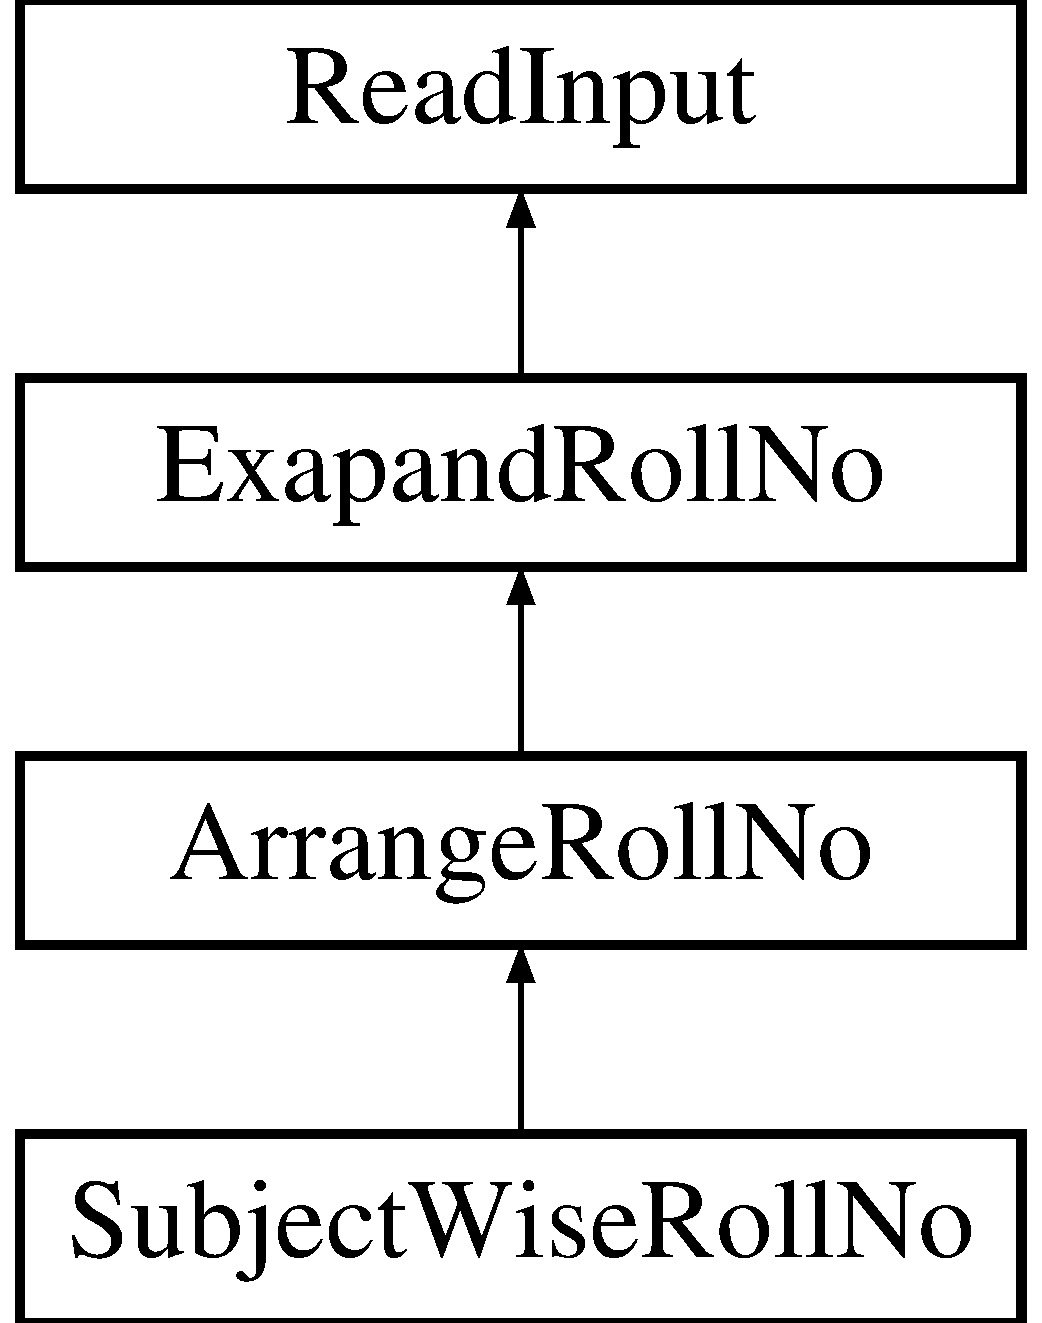
\includegraphics[height=4.000000cm]{classSubjectWiseRollNo}
\end{center}
\end{figure}
\subsection*{Public Member Functions}
\begin{DoxyCompactItemize}
\item 
\hypertarget{classSubjectWiseRollNo_aface8a14361aeeb9a6127d98d60e7732}{void {\bfseries subject\-Wise\-Roll\-No} ()}\label{classSubjectWiseRollNo_aface8a14361aeeb9a6127d98d60e7732}

\item 
\hypertarget{classSubjectWiseRollNo_a243121bce1807bada075e686f740643f}{void {\bfseries set\-Sub\-Code} ()}\label{classSubjectWiseRollNo_a243121bce1807bada075e686f740643f}

\item 
\hypertarget{classSubjectWiseRollNo_acfe5a3d07cad3397efd866fb87b54db7}{void {\bfseries remove\-Redundant\-Sub\-Code} ()}\label{classSubjectWiseRollNo_acfe5a3d07cad3397efd866fb87b54db7}

\item 
\hypertarget{classSubjectWiseRollNo_adb376b81d6b5005889653332a064c977}{void {\bfseries show\-Subject\-Wise\-Roll\-No} ()}\label{classSubjectWiseRollNo_adb376b81d6b5005889653332a064c977}

\item 
\hypertarget{classSubjectWiseRollNo_aeeb07726ddfc0ec17fa8a02c5cd2ffff}{void {\bfseries Main} ()}\label{classSubjectWiseRollNo_aeeb07726ddfc0ec17fa8a02c5cd2ffff}

\end{DoxyCompactItemize}
\subsection*{Protected Attributes}
\begin{DoxyCompactItemize}
\item 
\hypertarget{classSubjectWiseRollNo_aa719b1f10268b6cc741132aced93a321}{int {\bfseries total\-\_\-code}}\label{classSubjectWiseRollNo_aa719b1f10268b6cc741132aced93a321}

\item 
\hypertarget{classSubjectWiseRollNo_a9700a22dff37ac2fd095cbcc3f3e2874}{int {\bfseries sub\-\_\-totalrno} \mbox{[}M\-I\-N\-\_\-\-S\-I\-Z\-E\mbox{]}}\label{classSubjectWiseRollNo_a9700a22dff37ac2fd095cbcc3f3e2874}

\item 
\hypertarget{classSubjectWiseRollNo_a9eef1e17ae0aace37af78b15395ee3e5}{int {\bfseries subject\-\_\-size}}\label{classSubjectWiseRollNo_a9eef1e17ae0aace37af78b15395ee3e5}

\item 
\hypertarget{classSubjectWiseRollNo_a3e21660fe01181bf4595c4fe2163c528}{string {\bfseries sub\-\_\-subcode} \mbox{[}M\-I\-N\-\_\-\-S\-I\-Z\-E\mbox{]}}\label{classSubjectWiseRollNo_a3e21660fe01181bf4595c4fe2163c528}

\item 
\hypertarget{classSubjectWiseRollNo_a20ba02f66c6a634c1f4daeb0bd27b481}{string {\bfseries sub\-\_\-rollno} \mbox{[}M\-I\-N\-\_\-\-S\-I\-Z\-E\mbox{]}\mbox{[}M\-A\-X\-\_\-\-S\-I\-Z\-E\mbox{]}}\label{classSubjectWiseRollNo_a20ba02f66c6a634c1f4daeb0bd27b481}

\end{DoxyCompactItemize}


The documentation for this class was generated from the following files\-:\begin{DoxyCompactItemize}
\item 
Baka\-Plan/\-Seat\-Plan/subject-\/wise-\/rollno.\-h\item 
Baka\-Plan/\-Seat\-Plan/subject-\/wise-\/rollno.\-cc\end{DoxyCompactItemize}

\hypertarget{classValidation}{\section{Validation Class Reference}
\label{classValidation}\index{Validation@{Validation}}
}
Inheritance diagram for Validation\-:\begin{figure}[H]
\begin{center}
\leavevmode
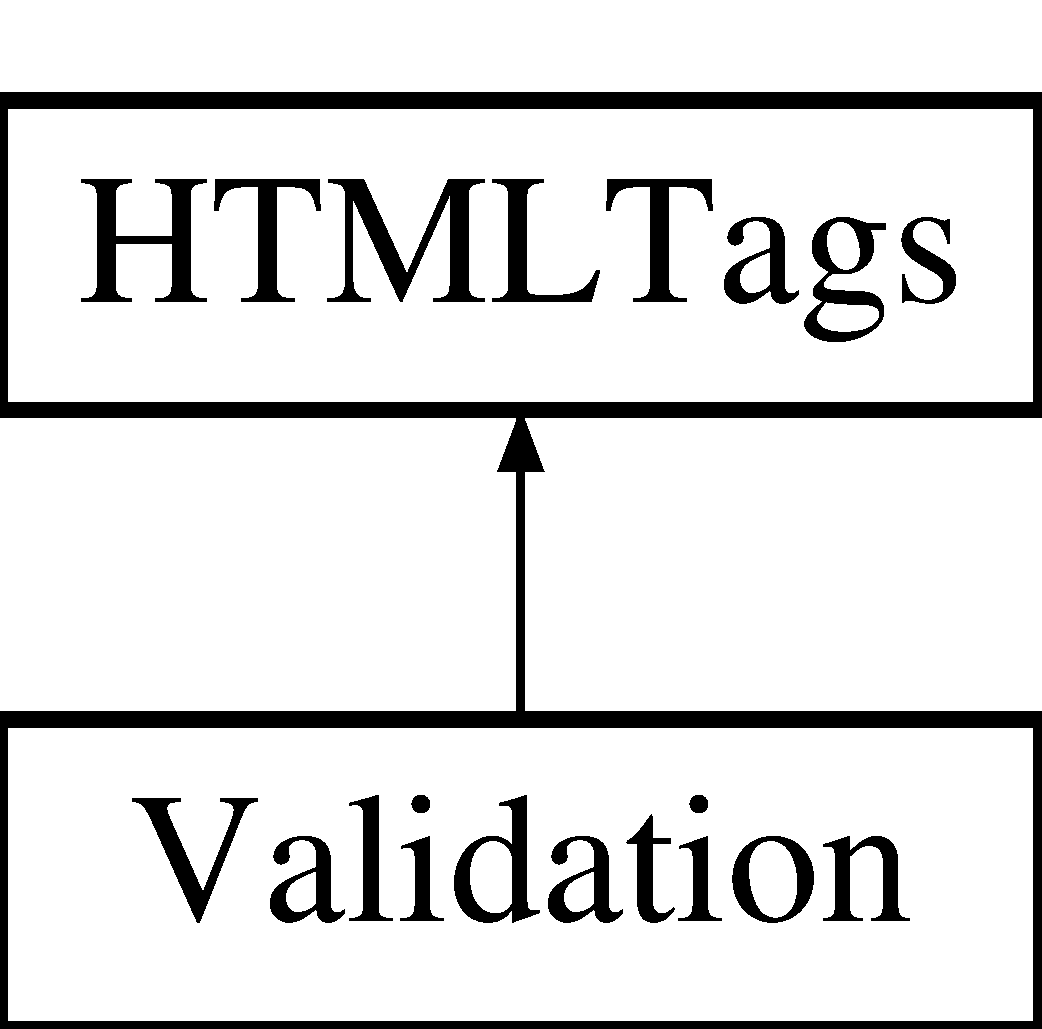
\includegraphics[height=2.000000cm]{classValidation}
\end{center}
\end{figure}
\subsection*{Public Member Functions}
\begin{DoxyCompactItemize}
\item 
\hypertarget{classValidation_a819164fd5c442a00234c711a52058183}{void {\bfseries Head} ()}\label{classValidation_a819164fd5c442a00234c711a52058183}

\item 
\hypertarget{classValidation_ab5ef950f034480d2d816f29931b9b1d6}{void {\bfseries Javascript} ()}\label{classValidation_ab5ef950f034480d2d816f29931b9b1d6}

\item 
\hypertarget{classValidation_a6be2c2abf5c3b046f0e66b6a59bd43b6}{void {\bfseries Body} ()}\label{classValidation_a6be2c2abf5c3b046f0e66b6a59bd43b6}

\item 
\hypertarget{classValidation_ace0de6d89e636387f1a3663df6850b2e}{void {\bfseries Body\-Content} ()}\label{classValidation_ace0de6d89e636387f1a3663df6850b2e}

\item 
\hypertarget{classValidation_a12a15d56dbb9ebce7f8675b5ae828524}{void {\bfseries read\-Strategy} ()}\label{classValidation_a12a15d56dbb9ebce7f8675b5ae828524}

\item 
\hypertarget{classValidation_a646be001379f091a4c9f38d9e784ab75}{void {\bfseries Main} ()}\label{classValidation_a646be001379f091a4c9f38d9e784ab75}

\end{DoxyCompactItemize}
\subsection*{Protected Attributes}
\begin{DoxyCompactItemize}
\item 
\hypertarget{classValidation_a1313f03a0092ea1d882a60fecaa58e67}{string {\bfseries strategy\-Choice}}\label{classValidation_a1313f03a0092ea1d882a60fecaa58e67}

\item 
\hypertarget{classValidation_a4224a467d43a9df314a78ee22061d8d6}{Cgicc {\bfseries form\-Data}}\label{classValidation_a4224a467d43a9df314a78ee22061d8d6}

\item 
\hypertarget{classValidation_abc319ff9dba2f9d78f68a825c345d093}{form\-\_\-iterator {\bfseries fi}}\label{classValidation_abc319ff9dba2f9d78f68a825c345d093}

\end{DoxyCompactItemize}


The documentation for this class was generated from the following files\-:\begin{DoxyCompactItemize}
\item 
validation.\-h\item 
validation.\-cc\end{DoxyCompactItemize}

\printindex
\end{document}
